\documentclass{vkr}
\usepackage[english, russian]{babel} % переносы
\usepackage{graphicx} % для вставки картинок
\graphicspath{{images/}} % путь к изображениям
\usepackage[hidelinks]{hyperref}
\usepackage{float} % определяет метод H для рисунка с переносом на следующую страницу, ели не помещается
\usepackage{pdflscape}
\addto{\captionsrussian}{\renewcommand{\refname}{СПИСОК ИСПОЛЬЗОВАННЫХ ИСТОЧНИКОВ}}
\usepackage{xltabular} % для вставки таблиц
\usepackage{makecell}
\renewcommand\theadfont{} % шрифт в /thead
\usepackage{array} % для определения новых типов столбцов таблиц
\newcolumntype{T}{>{\centering\arraybackslash}X} % новый тип столбца T - автоматическая ширина столбца с выравниванием по центру
\newcolumntype{R}{>{\raggedleft\arraybackslash}X} % новый тип столбца R - автоматическая ширина столбца с выравниванием по правому краю
\newcolumntype{C}[1]{>{\centering\let\newline\\\arraybackslash\hspace{0pt}}m{#1}} % новый тип столбца C - фиксированная ширина столбца с выравниванием по центру
\newcolumntype{r}[1]{>{\raggedleft\arraybackslash}p{#1}} % новый тип столбца r - фиксированная ширина столбца с выравниванием по правому краю
\newcommand{\centrow}{\centering\arraybackslash} % командой \centrow можно центрировать одну ячейку (заголовок) в столбце типа X или p, оставив в оcтальных ячейках другой тип выравнивания
\newcommand{\finishhead}{\endhead\hline\endlastfoot}
\newcommand{\continuecaption}[1]{\captionsetup{labelformat=empty} \caption[]{#1}\\ \hline }
\usepackage{etoolbox}
\AtBeginEnvironment{xltabular}{\refstepcounter{tablecnt}} % подсчет таблиц xltabular, обычные таблицы подсчитываются в классе

\usepackage[tableposition=top]{caption} % подпись таблицы вверху
\captionsetup{strut=off}
\setlength{\intextsep}{0pt} % Vertical space above & below [h] floats
\setlength{\textfloatsep}{0pt} % Vertical space below (above) [t] ([b]) floats
\DeclareCaptionLabelFormat{gostfigure}{Рисунок #2} %подпись рисунка
\DeclareCaptionLabelFormat{gosttable}{Таблица #2} %подпись таблицы
\DeclareCaptionLabelSeparator{gost}{~--~} %разделитель в рисунках и таблицах
\captionsetup{labelsep=gost}
\captionsetup[figure]{aboveskip=10pt,belowskip=4mm,justification=centering,labelformat=gostfigure} % настройка подписи рисунка
\captionsetup[table]{font={stretch=1.41},skip=0pt,belowskip=0pt,aboveskip=8.5pt,singlelinecheck=off,labelformat=gosttable} % настройка подписи таблицы

\setlength{\LTpre}{8mm} % отступ сверху таблицы
\setlength{\LTpost}{6mm} % отступ снизу таблицы

\usepackage{enumitem}
\setlist{nolistsep,wide=\parindent,itemindent=*} % отступы вокруг списков, выравнивание с учетом разделителя

\usepackage{color} %% это для отображения цвета в коде
\usepackage{listings} %% листинги кода
\setmonofont[Scale=0.7]{Verdana} % моноширный шрифт для листинга

\definecolor{codegreen}{rgb}{0,0.6,0}
\definecolor{codegray}{rgb}{0.5,0.5,0.5}
\definecolor{codepurple}{rgb}{0.58,0,0.82}

\lstset{ %
language=C,                 % выбор языка для подсветки (здесь это С)
numbers=left,               % где поставить нумерацию строк (слева\справа)
numberstyle=\tiny,           % размер шрифта для номеров строк
stepnumber=1,                   % размер шага между двумя номерами строк
numbersep=5pt,                % как далеко отстоят номера строк от подсвечиваемого кода
commentstyle=\color{codegreen},
keywordstyle=\color{magenta},
numberstyle=\tiny\color{codegray},
stringstyle=\color{codepurple},
basicstyle=\linespread{0.95}\ttfamily,
backgroundcolor=\color{white}, % цвет фона подсветки - используем \usepackage{color}
showspaces=false,            % показывать или нет пробелы специальными отступами
showstringspaces=false,      % показывать или нет пробелы в строках
showtabs=false,             % показывать или нет табуляцию в строках
frame=single,              % рисовать рамку вокруг кода
tabsize=2,                 % размер табуляции по умолчанию равен 2 пробелам
captionpos=t,              % позиция заголовка вверху [t] или внизу [b] 
breaklines=true,           % автоматически переносить строки (да\нет)
breakatwhitespace=false, % переносить строки только если есть пробел
escapeinside={\%*}{*)}   % если нужно добавить комментарии в коде
}

\makeatletter % чтобы допускались русские комментарии в листингах
\lst@InputCatcodes
\def\lst@DefEC{%
 \lst@CCECUse \lst@ProcessLetter
  ^^80^^81^^82^^83^^84^^85^^86^^87^^88^^89^^8a^^8b^^8c^^8d^^8e^^8f%
  ^^90^^91^^92^^93^^94^^95^^96^^97^^98^^99^^9a^^9b^^9c^^9d^^9e^^9f%
  ^^a0^^a1^^a2^^a3^^a4^^a5^^a6^^a7^^a8^^a9^^aa^^ab^^ac^^ad^^ae^^af%
  ^^b0^^b1^^b2^^b3^^b4^^b5^^b6^^b7^^b8^^b9^^ba^^bb^^bc^^bd^^be^^bf%
  ^^c0^^c1^^c2^^c3^^c4^^c5^^c6^^c7^^c8^^c9^^ca^^cb^^cc^^cd^^ce^^cf%
  ^^d0^^d1^^d2^^d3^^d4^^d5^^d6^^d7^^d8^^d9^^da^^db^^dc^^dd^^de^^df%
  ^^e0^^e1^^e2^^e3^^e4^^e5^^e6^^e7^^e8^^e9^^ea^^eb^^ec^^ed^^ee^^ef%
  ^^f0^^f1^^f2^^f3^^f4^^f5^^f6^^f7^^f8^^f9^^fa^^fb^^fc^^fd^^fe^^ff%
  ^^^^20ac^^^^0153^^^^0152%
  % Basic Cyrillic alphabet coverage
  ^^^^0410^^^^0411^^^^0412^^^^0413^^^^0414^^^^0415^^^^0416^^^^0417%
  ^^^^0418^^^^0419^^^^041a^^^^041b^^^^041c^^^^041d^^^^041e^^^^041f%
  ^^^^0420^^^^0421^^^^0422^^^^0423^^^^0424^^^^0425^^^^0426^^^^0427%
  ^^^^0428^^^^0429^^^^042a^^^^042b^^^^042c^^^^042d^^^^042e^^^^042f%
  ^^^^0430^^^^0431^^^^0432^^^^0433^^^^0434^^^^0435^^^^0436^^^^0437%
  ^^^^0438^^^^0439^^^^043a^^^^043b^^^^043c^^^^043d^^^^043e^^^^043f%
  ^^^^0440^^^^0441^^^^0442^^^^0443^^^^0444^^^^0445^^^^0446^^^^0447%
  ^^^^0448^^^^0449^^^^044a^^^^044b^^^^044c^^^^044d^^^^044e^^^^044f%
  ^^^^0401^^^^0451%
  %%%
  ^^00}
\lst@RestoreCatcodes
\makeatother


% Режим шаблона (должен быть включен один из трех)
\ВКРtrue
%\Практикаtrue
%\Курсоваяtrue

\newcommand{\Дисциплина}{<<Проектирование и архитектура программных систем>>} % для курсовой
\newcommand{\КодСпециальности}{09.03.04} % Курсовая
\newcommand{\Специальность}{Программная инженерия} % Курсовая
\newcommand{\Тема}{Программное обеспечение для системы контроля и} % ВКР Курсовая
\newcommand{\ТемаВтораяСтрока}{управления доступом на круизном судне}
\newcommand{\ГдеПроводитсяПрактика}{Юго-Западном государственном университете} % для практики
\newcommand{\РуководительПрактПредпр}{} % для практики
\newcommand{\ДолжнРуководительПрактПредпр}{директор} % для практики
\newcommand{\РуководительПрактУнивер}{Чаплыгин А. А.} % для практики
\newcommand{\ДолжнРуководительПрактУнивер}{к.т.н. доцент} % для практики
\newcommand{\Автор}{Д.Д.Дараган}
\newcommand{\АвторРод}{Дарагана Д.Д.}
\newcommand{\АвторПолностьюРод}{Дарагана Даниила Дмитриевича} % для практики
\newcommand{\Шифр}{20-06-0258}
\newcommand{\Курс}{4} % для практики
\newcommand{\Группа}{ПО-02б}
\newcommand{\Руководитель}{Е. И. Аникина} % для ВКР и курсовой
\newcommand{\Нормоконтроль}{А. А. Чаплыгин} % для ВКР
\newcommand{\ЗавКаф}{А. В. Малышев} % для ВКР
\newcommand{\ДатаПриказа}{«15» апреля 2024~г.} % для ВКР
\newcommand{\НомерПриказа}{1616-с} % для ВКР
\newcommand{\СрокПредоставления}{«11» июня 2024~г.} % для ВКР, курсового

\begin{document}
\maketitle
\ifПрактика{}\else{
   \newpage
\begin{center}
\large\textbf{Минобрнауки России}

\large\textbf{Юго-Западный государственный университет}
\vskip 1em
\normalsize{Кафедра программной инженерии}
\vskip 1em
\ifВКР{
        \begin{flushright}
        \begin{tabular}{p{.4\textwidth}}
        \centrow УТВЕРЖДАЮ: \\
        \centrow Заведующий кафедрой \\
        \hrulefill \\
        \setarstrut{\footnotesize}
        \centrow\footnotesize{(подпись, инициалы, фамилия)}\\
        \restorearstrut
        «\underline{\hspace{1cm}}»
        \underline{\hspace{3cm}}
        20\underline{\hspace{1cm}} г.\\
        \end{tabular}
        \end{flushright}
        }\fi
\end{center}
\vspace{1em}
  \begin{center}
  \large
\ifВКР{
ЗАДАНИЕ НА ВЫПУСКНУЮ КВАЛИФИКАЦИОННУЮ РАБОТУ
  ПО ПРОГРАММЕ БАКАЛАВРИАТА}
  \else
ЗАДАНИЕ НА КУРСОВУЮ РАБОТУ (ПРОЕКТ)
\fi
\normalsize
  \end{center}
\vspace{1em}
{\parindent0pt
  Студента \АвторРод, шифр\ \Шифр, группа \Группа
  
1. Тема «\Тема\ \ТемаВтораяСтрока»
\ifВКР{
утверждена приказом ректора ЮЗГУ от \ДатаПриказа\ № \НомерПриказа
}\fi.

2. Срок предоставления работы к защите \СрокПредоставления

3. Исходные данные для создания программной системы:

3.1. Перечень решаемых задач:}

\renewcommand\labelenumi{\theenumi)}

\begin{enumerate}
\item исследовать и проанализировать предметную область
\item спроектировать базу данных для будущей системы
\item сконструировать базу данных в соответствии с бизнес-правилами системы
\item заполнить базу данными, отражающими отношения внутри базы данных
\item сконструировать программную систему контроля и управления доступом на круизном судне
\item протестировать программную систему
\end{enumerate}

{\parindent0pt
  3.2. Входные данные и требуемые результаты для программы:}

\begin{enumerate}
\item Входными данными для программной системы являются: личные данные пользователей, отдыхающих на круизном судне; данные о наложенных штрафах и ограничениях; конфигурации дверей, к которым запрашивается доступ; данные о ситуации на судне.
\item Выходными данными для программной системы являются: данные каждой таблицы базы в формате набора полей, содержимое которых можно просматривать, изменять и удалять; данные о доступах каждого пассажира к каждой двери на круизном лайнере с учётом текущей ситуации на судне.
ИТ-ресурсов, воронка заявок.
\end{enumerate}

{\parindent0pt

  4. Содержание работы (по разделам):
  
  4.1. Введение
  
  4.1. Анализ предметной области
  
4.2. Техническое задание: основание для разработки, назначение разработки, требования к интерфейсу,
требования к программной системе, построение ER-модели, нефункциональные требования к программной системе, требования к оформлению документации.

4.3. Технический проект: общая характеристика организации решения задачи, общие сведения о программной системе, основание выбора технологии проектирования, диаграмма размещения, описание архитектуры программной системы, проектирование пользовательского интерфейса программной системы.

4.4. Рабочий проект: спецификация компонентов и классов программной системы, тестирование программной системы, сборка компонентов программной системы.

4.5. Заключение

4.6. Список использованных источников

5. Перечень графического материала: ...

\списокПлакатов

\vskip 2em
\begin{tabular}{p{6.8cm}C{3.8cm}C{4.8cm}}
Руководитель \ifВКР{ВКР}\else работы (проекта) \fi & \lhrulefill{\fill} & \fillcenter\Руководитель\\
\setarstrut{\footnotesize}
& \footnotesize{(подпись, дата)} & \footnotesize{(инициалы, фамилия)}\\
\restorearstrut
Задание принял к исполнению & \lhrulefill{\fill} & \fillcenter\Автор\\
\setarstrut{\footnotesize}
& \footnotesize{(подпись, дата)} & \footnotesize{(инициалы, фамилия)}\\
\restorearstrut
\end{tabular}
}

\renewcommand\labelenumi{\theenumi.}

   \abstract{РЕФЕРАТ}

Объем работы равен \formbytotal{lastpage}{страниц}{е}{ам}{ам}. Работа содержит \formbytotal{figurecnt}{иллюстраци}{ю}{и}{й}, \formbytotal{tablecnt}{таблиц}{у}{ы}{}, \arabic{bibcount} библиографических источников и \formbytotal{числоПлакатов}{лист}{}{а}{ов} графического материала. Количество приложений – 2. Графический материал представлен в приложении А. Фрагменты исходного кода представлены в приложении Б.

Перечень ключевых слов: коммерческий сайт, Система, CMS, Битрикс, Joomla, аддитивные технологии, 3D-принтеры, услуги, сервисы, информатизация, автоматизация, информационные технологии, веб-форма,  Apache, классы, база данных, средства защиты информации, подсистема, компонент, модуль, сущность, информационный блок, метод, контент-редактор, администратор, пользователь, web-сайт.

Объектом разработки является web-сайт компании,  занимающейся производством 3D-принтеров, выпуском оборудования для создания порошков, разработкой программного обеспечения и организацией центров аддитивного производства.

Целью выпускной квалификационной работы является привлечение клиентов, увеличение заказов, информирование о продукции и услугах путем создания сайта компании.

В процессе создания сайта были выделены основные сущности путем создания информационных блоков, использованы классы и методы модулей, обеспечивающие работу с сущностями предметной области, а также корректную работу web-сайта, разработаны разделы, содержащие информацию о компании, ее деятельности, производимой продукции и услугах, разработан сервис по заказу 3D-деталей.

При разработке сайта использовалась система управления контентом "<1С-Битрикс: Управление сайтом">.

Разработанный сайт был успешно внедрен в компании.

\selectlanguage{english}
\abstract{ABSTRACT}
  
The volume of work is \formbytotal{lastpage}{page}{}{s}{s}. The work contains \formbytotal{figurecnt}{illustration}{}{s}{s}, \formbytotal{tablecnt}{table}{}{s}{s}, \arabic{bibcount} bibliographic sources and \formbytotal{числоПлакатов}{sheet}{}{s}{s} of graphic material. The number of applications is 2. The graphic material is presented in annex A. The layout of the site, including the connection of components, is presented in annex B.

List of keywords: commercial website, System, CMS, Bitrix, Joomla, additive technologies, 3D printers, services, services, informatization, automation, information technology, web form, Apache, classes, database, component, module, entity, information block, method, content editor, administrator, user, web site.

The object of the research is the analysis of information technologies for the development of a production company's website.

The object of the development is the website of a company engaged in the production of 3D printers, the production of equipment for the creation of powders, software development and the organization of additive manufacturing centers.

The purpose of the final qualifying work is to attract customers, increase orders, inform about products and services by creating a company website.

In the process of creating the site, the main entities were identified by creating information blocks, classes and methods of modules were used to ensure work with the entities of the subject area, as well as the correct operation of the website, sections containing information about the company, its activities, products and services were developed, a service for ordering 3D parts was developed.

When developing the site, the content management system <<1C – Bitrix: Site Management>> was used.

The developed website was successfully implemented in the company.
\selectlanguage{russian}
}\fi
\tableofcontents
\section*{ОБОЗНАЧЕНИЯ И СОКРАЩЕНИЯ}

БД -- база данных.

ИС -- информационная система.

ИТ -- информационные технологии. 

UI - User Interface, пользовательский интерфейс.

ООП - объектно-ориентированное программирование.

ПО -- программное обеспечение.

РП -- рабочий проект.

СУБД -- система управления базами данных.

ТЗ -- техническое задание.

ТП -- технический проект.

CRUD - Create, Read, Update, Delete, основные операции для работы с данными.

ER (Entity-Relationship model) -- модель данных, позволяющая описывать концептуальные схемы предметной области. ER-модель используется при высокоуровневом (концептуальном) проектировании баз данных.

СКУД -- система контроля и управления доступом.

УД -- учётные данные.

ЧС -- чрезвычайная ситуация.

PkID(Primary key Identifier, первичный ключ) -- в реляционной модели данных один из потенциальных ключей отношения, выбранный в качестве основного ключа (или ключа по умолчанию).

UID(Unique identifier, уникальный идентификатор) -- идентификатор, который используют для однозначного определения объекта, однако признак уникальности не заложен в ID.

FKID(Foreign key identifier, внешний ключ) -- идентификатор, который применяется для принудительного установления связи между данными в двух таблицах с целью контроля данных, которые могут храниться в таблице внешнего ключа.

TreeView -- элемент графического интерфейса для иерархического отображения информации. Представляет собой совокупность связанных отношениями структуры пиктограмм в иерархическом древе.
\ifПрактика{}\else{\section*{ВВЕДЕНИЕ}
\addcontentsline{toc}{section}{ВВЕДЕНИЕ}

Аддитивные технологии (АТ) начали активно развиваться со времени получения первых трехмерных изображений изделий на дисплеях компьютеров. Начало положила стереолитография, затем довольно многочисленные новые принципы стали называть технологиями быстрого прототипирования, затем укоренилось название "<Аддитивные технологии">. Интенсивность развития данных технологий не имеет аналогов. АТ изменили процессы проектирования и конструирования изделий, превратив их в процессы непрерывного создания изделий. Современные проектирование и производство изделий невозможно представить без данного рода технологий. 3D-принтеры стали такими же распространенными, как и персональные компьютеры. С помощью 3D-принтеров получают ткани, обувь, продукты питания, а также выращивают человеческие органы. Во многих отраслях, например, в космической отрасли, альтернативы аддитивным технологиям нет.

АТ предполагают изготовление детали методом послойного нанесения материала, в отличие от традиционных методов формирования детали, за счёт удаления материала из массива заготовки.

При использовании АТ все стадии реализации проекта от идеи до материализации находятся в единой технологической цепи, в которой каждая технологическая операция выполняется в цифровой CAD/CAM/CAE-системе.

Современные компании, видя, как развиваются информационные технологии, пытаются использовать их выгодно для своего бизнеса, поэтому запускают свой web-сайт. С его помощью предприятие может заявить о себе, проинформировать потенциального заказчика об услугах или продуктах, которые предоставляет, а также позволяет пользователям сделать с помощью сайта онлайн-заказ, произвести покупку или оплатить счета.

Сайт считается лицом компании и может существенно повысить ее имидж. Любой пользователь сети Интернет сможет получить необходимую информацию о компании в любой момент, появляется возможность найти контактные телефоны, адрес и e-mail, чтобы связаться с компанией. Сейчас большинство клиентов узнают о ее существовании именно через сайт. Поэтому сайт можно назвать самой лучшей рекламой. 

Главной задачей профессионально построенного сайта является превращение посетителя, зашедшего на сайт, в потенциального клиента.

\emph{Цель настоящей работы} – разработка web-сайта компании для привлечения новой аудитории, увеличения заказов, рекламы продукции и услуг компании. Для достижения поставленной цели необходимо решить \emph{следующие задачи:}
\begin{itemize}
\item провести анализ предметной области;
\item разработать концептуальную модель web-сайта;
\item спроектировать web-сайт;
\item реализовать сайт средствами web-технологий.
\end{itemize}

\emph{Структура и объем работы.} Отчет состоит из введения, 4 разделов основной части, заключения, списка использованных источников, 2 приложений. Текст выпускной квалификационной работы равен \formbytotal{page}{страниц}{е}{ам}{ам}.

\emph{Во введении} сформулирована цель работы, поставлены задачи разработки, описана структура работы, приведено краткое содержание каждого из разделов.

\emph{В первом разделе} на стадии описания технической характеристики предметной области приводится сбор информации о деятельности компании, для которой осуществляется разработка сайта.

\emph{Во втором разделе} на стадии технического задания приводятся требования к разрабатываемому сайту.

\emph{В третьем разделе} на стадии технического проектирования представлены проектные решения для web-сайта.

\emph{В четвертом разделе} приводится список классов и их методов, использованных при разработке сайта, производится тестирование разработанного сайта.

В заключении излагаются основные результаты работы, полученные в ходе разработки.

В приложении А представлен графический материал.
В приложении Б представлены фрагменты исходного кода. 
}\fi
\section{Анализ предметной области}
\subsection{Характеристика СКУД и её назначение}

Сегодня под термином СКУД (Система контроля и управления доступом) понимается вид физической безопасности, который управляет точками входа в ваш бизнес или внутренние помещения здания. Простой пример СКУД -- ворота, физически не допускающие неавторизованных пользователей и позволяющие войти только авторизованным пользователям.

Минимальная функциональность СКУД – проверка наличия кода в базе данных и, при положительном результате, выполнение разблокировки преграждающего устройства. Однако в настоящее время существует некий «джентльменский набор» выполняемых действий, которые должны быть реализованы в любой уважающей себя СКУД – это контроль кого, куда и когда пускать.

В некоторых случаях к этому набору добавляются функции запрета повторного прохода (запрет на повторный вход, если не было выхода) и запрет прохода во внутренние помещения без пересечения проходной (внешнего периметра).

В большинстве случаев профессиональные СКУД обеспечивают и иные режимы проходов, например, проход по двум ключам,  шлюз, контрольный обход территории, дисциплина проходов во внутренние зоны.

Три лидера отрасли в РФ, каждый из которых разработал инновационные системы контроля доступа -- <<АAМ Системз>>, <<Равелин>> и <<PERCo>> разрабатывают передовые системы безопасности, которые являются универсальными, масштабируемыми и гибкими, оставаясь при этом высокофункциональными.
%Актуальность данной темы заключается в необходимости установки порядка и правил на объекте с большим количеством людей, минимизации влияния ручного управления на систему, а также сокращении расходов на персонал, занимающий потенциальные места для продажи.

\subsection{Ключевые элементы системы контроля доступа и принцип их работы}
\subsubsection{Учётные данные}

Учетные данные контроля доступа используют RFID (радиочастотную идентификацию) для передачи сигналов на панель контроля доступа. Каждая метка имеет уникальный зашифрованный идентификационный номер. Владелец системы может выдать всем сотрудникам метки одного типа, но при этом настроить одну метку на разрешение входа, а другую - на запрет входа в определенные зоны здания.

УД бывают следующих видов:

\begin{itemize}
	\item пароль или пин-код;
	\item биометрия.
\end{itemize}


\paragraph{Пароль или ПИН-код}

Преимущество парольных систем по сравнению с системами дискреционного контроля доступа на основе матрицы доступа заключается в том, что в них нет объекта, связанного с монитором безопасности, который хранит информацию о контроле доступа к конкретным объектам. Кроме того, парольные системы обеспечивают безопасность даже в том случае, если посторонние лица имеют неограниченный или технически возможный доступ к носителям, на которых записаны и хранятся зашифрованные объекты. Эти преимущества парольных систем управления доступом делают их чрезвычайно распространенными в документальных информационных системах.

\paragraph{Биометрия}

Объекты со строгими требованиями к соблюдению норм и правил, такие как больницы и производственные предприятия, требуют особенно надежных систем контроля доступа и безопасности. Биометрические технологии используют измерения тела и физические характеристики для поиска уникальных идентификационных признаков человека (обычно отпечатков пальцев, сканирования сетчатки глаза или лица), чтобы сделать идентификацию положительной. 

\subsubsection{Устройства-носители данных}

Такие устройства выполняют идентичные функции, выступая носителями данных вместо пользователя.

Самыми распространёнными устройствами такого вида являются:

\begin{itemize}
	\item данные устройства;
	\item брелок или карта доступа.
\end{itemize}

\paragraph{Данные устройства}

Для контроля доступа с помощью мобильных устройств используются смартфоны, планшеты и носимые электронные устройства, которые служат удостоверением личности пользователя для входа в офис или другие деловые помещения. Поскольку большинство работодателей поощряют тенденцию Bring Your Own Device (BYOD), контроль доступа с помощью приложений стал одним из самых эффективных инструментов для обеспечения дополнительного уровня безопасности в любой организации. В настоящее время электронные устройства позволяют осуществлять биометрическую аутентификацию без необходимости инвестировать в дорогостоящие биометрические считыватели.

\paragraph{Брелок или карта доступа}

Карта доступа – это идентификатор пользователя, на котором содержится некая информация – ключ, открывающий дверь или доступ к ресурсам. 
Системы контроля доступа на основе карт играют важную роль в защите вашей собственности. Системы доступа без ключа - это эффективный и доступный способ обеспечить безопасность людей, помещений и данных. Карточные системы подходят для объектов любого типа - охраняемого склада, общежития или коммерческого здания.

\subsubsection{Устройство СКУД}

Базовая современная СКУД состоит из:

\begin{itemize}
	\item считывателя;
	\item контроллера;
	\item замка.
\end{itemize}

\paragraph {Считыватель}

Считыватель меток находится на одной или обеих сторонах двери - на одной стороне двери, если система контролирует только вход, или на обеих сторонах, если система контроля доступа контролирует вход и выход. Считыватель содержит антенну, которая подключается к панели контроля доступа и получает от нее питание.
Когда человек входит в здание со своей меткой контроля доступа, на антенну считывателя поступает его зашифрованный идентификационный номер.

\paragraph {Контроллер}

Контроллер - это ядро системы. В нем хранится информация об авторизации, которая настраивается администратором системы. Контроллер получает зашифрованный номер метки от считывателя, расшифровывает его, затем сравнивает ID-номер с ID-номерами, которые были загружены в систему. Если номера совпадают, и пользователь имеет право доступа к двери, дверь разблокируется.

\paragraph {Замок}

Панель управления доступом, или контроллер, управляет электрическим замком двери. Если пользователю разрешено войти в здание, дверь автоматически разблокируется и может быть открыта.
Общая схема устройства системы изображена на рисунке ~\ref{fig:commonscheme1}.
\begin{figure}
	\centering
	
\includegraphics[width=0.8\linewidth]{images/CommonScheme1}
	\caption{Схема устройства современной СКУД}
	\label{fig:commonscheme1}
\end{figure}

\subsubsection {СКУД на больших предприятиях}
В настоящее время, на больших охраняемых объектах строение СКУД значительно отличается от представленного выше и представляет из себя её многократно модифицированную версию. Так, СКУД, производимый Российской компанией \textquotedbl АВС Строй Защита \textquotedbl, изображенная на рисунке ~\ref{fig:bigskud}, иллюстрирует модель для СКУД для зданий предприятий:
\begin{itemize}
	\item уникальный компьютер-носитель бизнес-правил для каждой нетипичной территории объекта, подключенный по локальной сети к остальным;
	\item наличие в системе видеокамер;
	\item существование общего адаптера для подключения контроллеров к локальной сети.
\end{itemize}

\begin{figure}[H]
	\centering
	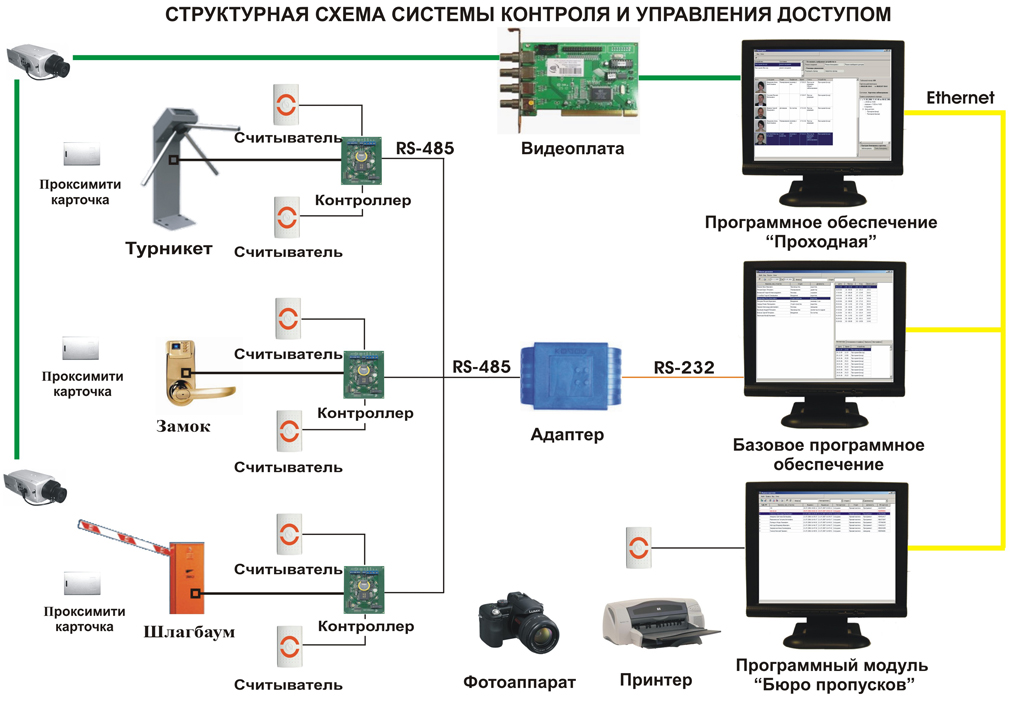
\includegraphics[width=1\linewidth]{images/BigSkud}
	\caption{Схема усовершенствованной СКУД для предприятий}
	\label{fig:bigskud}
\end{figure}

Некоторые компании предпочитают использовать клиент-серверное размещение системы вместо локальной сети. Такое решение расширяет спектр решений по повышению эффективности системы, однако делает её уязвимой для атак типа \textquotedbl SQL-инъекция \textquotedbl, что может нанести предприятию существенный ущерб.
\subsection{Анализ категорий пользователей СКУД}

Система контроля и управления доступом - неотъемлемая часть безопасности. Она обеспечивает дополнительный уровень защиты, позволяя контролировать и отслеживать тех, кто имеет доступ к объекту защиты.

СКУД применима в отраслях - в здравоохранении, корпоративном, образовательном и государственном секторах. Сегодня они применяются на различных объектах, таких как стационарные, долговременные и жилые учреждения, больницы, муниципалитеты, кондоминиумы, распределительные комплексы, малые и крупные предприятия, а также колледжи и университеты.

Среди пользователей программного обеспечения СКУД -- системные администраторы и специалисты по информационной безопасности, нанятые организацией с целью контроля правил системы, устранения неполадок, проведения аудитов безопасности, поддержания работоспособности, внесения изменений.

В нашем случае, на круизном лайнере, пользователем приложения является человек из экипажа, занимающийся внесением данных пассажиров в базу, наложением штрафов, созданием правил для входа в те или иные сектора, манипуляцией доступом во время ЧС и т.д.

\subsection{Перспективы развития}
В перспективе развития СКУД на круизном лайнере ключевым является масштабирование её возможностей. Помимо существующих возможностей продвинутых систем контроля и управления доступом, упомянутых в пункте 1.2.4, для самой системы это может быть увеличение быстродействия, расширение набора правил и ограничений, добавление умных систем обнаружения (камер) для фиксации нарушений и автоматического наложения штрафов, внедрение технической поддержки в реальном времени для нерядовых случаев, внедрение большего количества режимов работы (при различных чрезвычайных ситуациях должны действовать неодинаковые правила).

В перспективе развития ПО для СКУД, ключевым является наиболее точное отражение функций системы для воздействия на них со стороны специалиста.

В будущем может быть рассмотрена интеграция логики запросов в виде набора новых бизнес-правил, дополнительного уровня защиты базы данных от атак злоумышленников, а в интерфейсе пользователя – более широкую реализацию библиотек \textquotedbl tkinter \textquotedbl и \textquotedbl customtkinter \textquotedbl, что обеспечит более гибкое управление ресурсами и улучшит масштабируемость приложения.

Системы безопасности изменялись и дополнялись в течение многих лет, от веревок и деревянных замков до облачных систем и биометрии. Сейчас аутентификация работает повсеместно - от больших и надежных объектов до телефонов в карманах людей. При взгляде на будущие тенденции в области контроля доступа мы можем сделать вывод, что процессы инновации, интеграции и адаптивность необходимы, но не в ущерб безопасности. Будущее контроля доступа, в большей степени для предприятий, охватывает не только задачи защиты данных и ограничения доступа, а также позволяет делать процесс быстрее и с большей надежностью.   

\subsection{Особенности СКУД на пассажирском судне}
Цель работы - специализированная программная и информационная поддержка СКУД круизного судна.

СКУД на пассажирском или круизном судне работает нестатично -- решение о пропуске и отказе базируется на заданных заранее правилах доступа, соотвественно которым это решение может меняться на протяжении поездки. Основные правила выглядят следующим образом:
\begin{enumerate}
	\item Каждый человек на борту имеет постоянный доступ к жизненно-необходимым дверям:(коридорные и лестничные, туалет, собственный номер, столовая, выход на площадку, медпункт, детская комната.
	Однако, если помещение переполнено, действует режим ЧС(для площадок с открытым небом), пассажир пытается попасть в не соответствующий его полу туалет и т.д. -- в этом случае доступ не предоставляется.
	\item Предоставление доступа к некоторым комнатам действует по иерархической системе. Так, обладатели тарифа \textquotedbl Средний \textquotedbl к бару, аквапарку, кинотеатру, кальянной, бильярдной, банкетному залу, тиру.
	Однако, предоставлению доступа могут помешать иные ограничения, наложенные на комнату, в которую ведёт дверь. Это медицинские ограничения (аквапарк), ограничения по времени (банкетный зал), судимости (тир) и штрафы, накладываемые после проишествий.
	\item Персонал имеет доступ ко всем дверям, кроме личных номеров пассажиров.
	\item Пассажир может менять тариф в процессе путешествия. Это происходит в случае доплаты за услуги в процессе поедки (для повышения) и, в случае персонала, при отстранении от полномочий -- тариф меняется на \textquotedbl Эконом \textquotedbl.
	\item Штраф пассажира может быть снят, но только, если:
	\begin{itemize}
		\item штраф относится к снимаемым;
		\item прошли 1 сутки с момента наложения;
		\item пассажир заплатил выкуп за снятие штрафа или обжаловал его.
	\end{itemize}
	\item Каждый человек на борту должен иметь свой пропуск, их количество для каждого не должно превышать 1. Пользование чужим пропуском в штатном режиме влечёт за собой наложение неснимаемого штрафа типа \textquotedbl Обман системы\textquotedbl.
	\item Несовершеннолетние также имеют свой пропуск.
	Однако, для разблокировки пропуска за несовершеннолетним должен быть закреплён сопровождающий.
	\item Ограничения пассажира могут быть как постоянными, так и наоборот. К ограничениям, что не изменяются и не оспариваются во время поездки относятся:
	\begin{itemize}
		\item ограничения по здоровью;
		\item судимости;
		\item пол.
	\end{itemize}
	\item В рассчёт входят только те ограничения по судимостям, здоровью, возрасту, штрафам, полу, которые действительно противоречат доступу к комнате, находящейся за дверью. Система пропустит пассажира с проблемами в области сердца в тир, что не противоречит его показаниям. То, что с ним может случиться - уже его личная ответственность.
	\item У каждого пассажира должна быть своя комната. Пассажир может открыть только ту жилую комнату, что закреплена за ним.
	\item В случае возникновения ЧС, СКУД начинает работать в другом режиме.
	Например, в случае шторма все двери наружу закрываются, двери лестниц и коридоров всегда открыты для исключения ситуации давки.
	
\end{enumerate}  
\section{Техническое задание}
\subsection{Основание для разработки}

Полное наименование системы: «Программное обеспечение для системы контроля и управления доступом на круизном судне».
Основанием для разработки программы является приказ ректора ЮЗГУ от «15» апреля 2024 г. №1616-с «Об утверждении тем выпускных квалификационных работ».

\subsection{Цель и назначение разработки}

Целью данной работы является специализированная программная и информационная поддержка СКУД круизного судна.

В настоящее время перед СКУД стоят задачи: четкое и быстрое регулирование правил доступа во время поездки и обеспечение безопасной эвакуации пассажиров в случае ЧС. Для выполнения этих задач требуется систематизация данных. 

Основными задачами при проектировании и разработке базы данных  и приложения являются:
\begin{itemize}
	\item исследование предметной области;
	\item проектирование базы данных;
	\item создание базы данных;
	\item заполнение базы данных информацией;
	\item разработка  интерфейса;
	\item реализация приложения.
\end{itemize}

\subsection{Актуальность темы разработки}
Суда с древних времён служили одним из передовых способов переправки живых и неживых грузов на дальние расстояния по воде. Со временем, новые суда увеличивались в размерах, а следовательно, возрастала сложность управления и контроля этого вида транспорта. Это повлекло за собой необходимость увеличения количества людей, необходимых для поддержания стабильной и безопасной эксплуатации судна, обеспечения безопасности перевозимого груза и пассажиров в опасной морской среде.

Актуальность данной темы заключается в необходимости установки порядка и правил на объекте с большим количеством людей для их безопасности, минимизации влияния ручного управления на систему, а также сокращении расходов на персонал, занимающий потенциальные места для продажи.

\subsection{Требования к программной системе приложения <<СКУД на круизном лайнере>>}
\subsubsection{Требования к интерфейсу}

Приложение должно включать в себя:
\begin{itemize}
	\item навигацию по таблицам данных (Главное окно с возможностью выбрать таблицу по названию);
	\item страницу для работы с данными о пассажирах
	\item страницу для работы с данными о детях
	\item страницу для работы с данными о штрафах
	\item страницу для работы с данными о дверях
	\item страницу для работы с данными о комнатах
	\item страницу для отображения актуальных данных о доступе пассажиров к дверям с возможностью быстрой проверки наличия доступа у пассажира к двери в базе данных.
	\item отображение текущей таблицы данных в реальном времени(виджет TreeView для каждой таблицы данных);
	\item возможность так или иначе воздействовать на внесённые данные базы внутри приложения(напр. "Изменить элемент", "Удалить элемент", "Добавить элемент" и т.д.);
	\item понятную навигацию и легкий поиск среди элементов конкретной таблицы (Возможность перелистывать элемент в текущем окне отображения, поиск по полю ID);
	\item отображение локального времени во избежание ошибок;
\end{itemize}

\subsubsection{Требования к данным программной системы}

Система должна уметь эффективно обрабатывать данные пассажиров, включая личную информацию, данные о тарифе, информацию о штрафах и спутниках. Необходимо обеспечить конфиденциальность и безопасность этих данных.

Для работы СКУД в системе должна быть представлена информация о следуюших обьектах:

\begin{itemize}
	\item ДОСТУПЫ;
	\item ДОСТУПЫ-ЧС;
	\item ПАССАЖИРЫ;
	\item ДВЕРИ;
	\item КОМНАТЫ;
	\item ШТРАФЫ;
	\item ДЕТИ;
\end{itemize}


\subsection{Построение ER-модели данных}

Наборы объектов и связей в базе данных.

В приведенной на рисунке ~\ref{fig:er} ER-диаграмме представлены сущности и атрибуты, которые будут использоваться в программной системе 

\begin{figure}[ht]
	\centering
	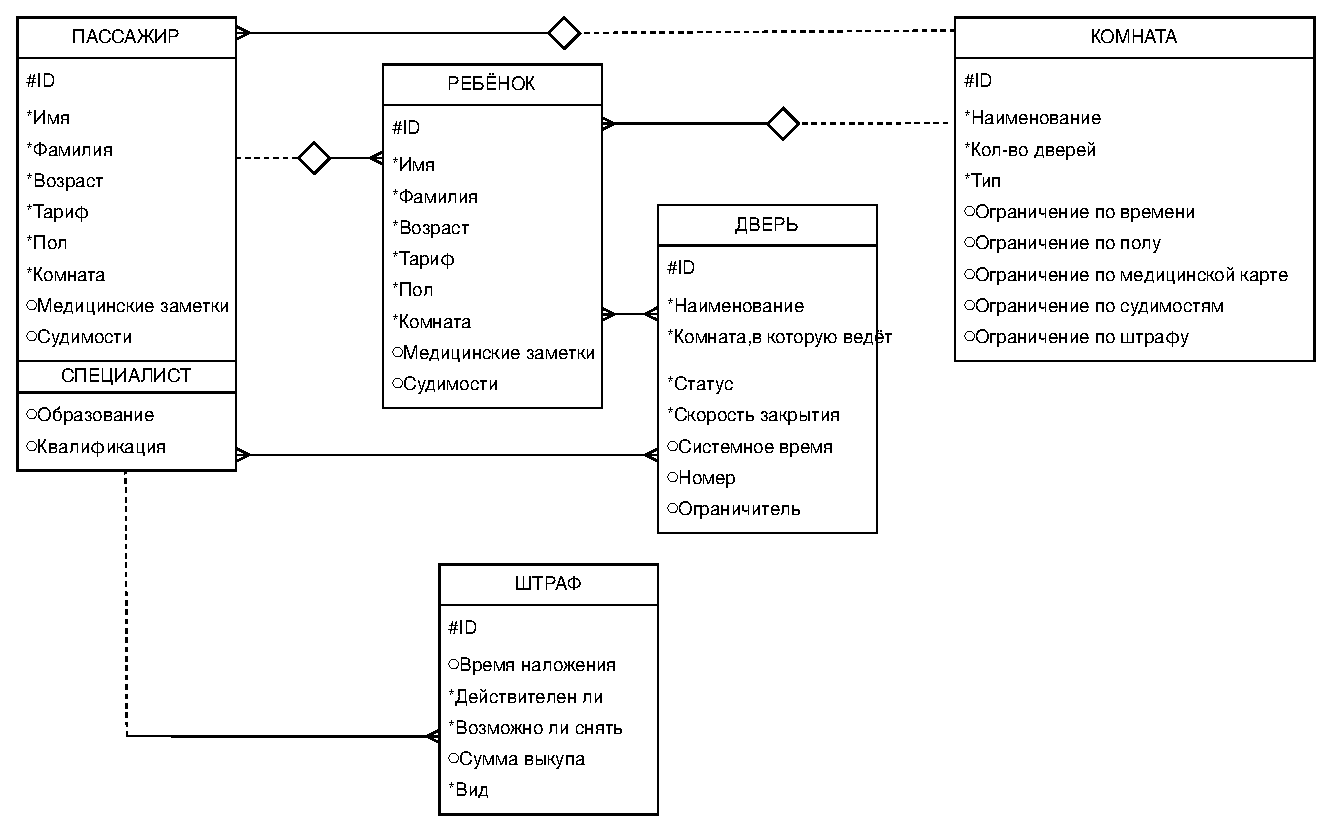
\includegraphics[width=1\linewidth]{images/ER}
	\caption{ER-диаграмма}
	\label{fig:er}
\end{figure}

\subsection{Функциональные требования к программной системе}

На основании анализа предметной области, разрабатываемая программная система «СКУД на круизном лайнере» должна включать в себя следующие ключевые функциональные возможности:
\begin{itemize}
	\item Открыть/закрыть таблицу
	\item Редактировать таблицу
	\item Перейти к следующему/предыдущему элементу
	\item Добавить новый элемент -- реализация опции добавления нового элемента с последующей актуализацией этих данных в БД 
	\item Редактировать выбранный элемент -- реализация опции редактирования элемента с последующей актуализацией этих данных в БД 
	\item Найти элемент по идентификатору
	\item Удалить элемент -- реализация опции редактирования элемента с последующей актуализацией этих данных в БД
	\item Запросить проверку доступа -- реализация опции запроса проверки пассажира на наличие доступа к двери
\end{itemize}

\subsection{Моделирование вариантов использования}

На рисунке  ~\ref{fig:commonscheme2} представлена диаграмма прецедентов, которая служит важным средством для систематизации функциональных требований и возможностей системы, выявляя ключевые сценарии использования. Диаграмма прецедентов изображает, как пользователи могут взаимодействовать с системой, а также помогает выявить набор основных функциональных возможностей, доступных пользователям.

При построении диаграммы вариантов использования применяется унифицированный язык визуального моделирования UML.

Каждый прецедент на диаграмме отражает отдельный путь взаимодействия в системе и представляет потенциальные действия, которые могут быть предприняты пользователями в различных ролях. Пользователем или действующим лицом является сущность, взаимодействующая с системой извне (например, человек, техническое устройство).

\begin{figure}[ht]
	\centering
	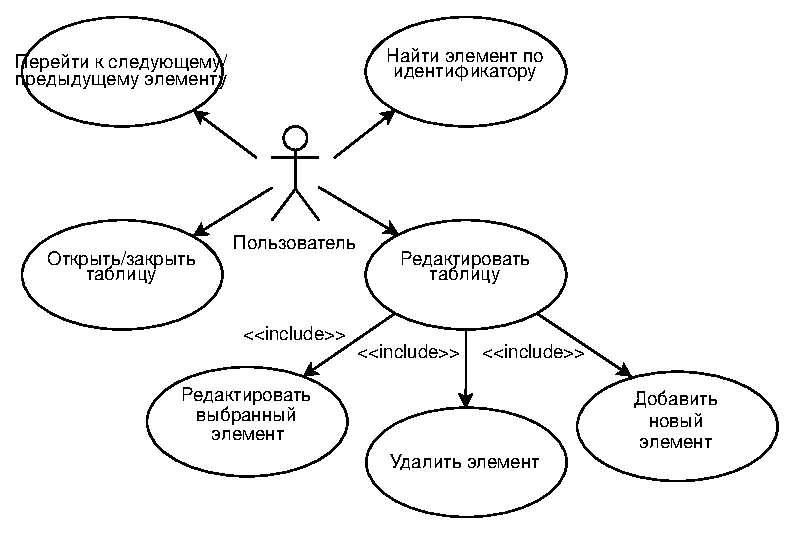
\includegraphics[width=1\linewidth]{images/CommonScheme2}
	\caption{Диаграмма прецедентов}
	\label{fig:commonscheme2}
\end{figure}

\subsubsection{Вариант использования <<Открыть/закрыть раздел данных>>}

Пользователь выбирает интересующую его раздел данных из списка предложенных и открывает окно, репрезентирующее требуемый от приложения интерфейс панели управления данными.
\subsubsection{Вариант использования <<Сменить режим работы>>}

На судне началась чрезвычайная ситуация и пользователь меняет режим работы СКУД в главном меню с помощью переключателя.

\subsubsection{Вариант использования <<Редактировать данныe>>}

Пользователь решает внести какие-либо изменения в данных. Он может сделать это, добавляя новые элементы, удаляя или редактируя существующие.

\subsubsection{Вариант использования <<Перейти к следующему/предыдущему элементу>>}

Пользователь листает элементы в таблице посредством перехода к предыдущему/следующему за текущим.

\subsubsection{Вариант использования <<Найти элемент по идентификатору>>}

Пользователь решает не листать элементы по одиночке т.к. не хочет тратить на это время. Он помнит идентификатор искомого элемента, вводит его в предназначенное текстовое поле и переходит к искомому элементу.

\subsubsection{Вариант использования <<Добавить новый элемент>>}

Пользователь заполняет поля данных будущего объекта и добавляет его в таблицу по клику.

\subsubsection{Вариант использования <<Редактировать выбранный элемент>>}

Пользователь редактирует необходимые ему поля у текущего элемента и вносит эти изменения в таблицу по клику.

\subsubsection{Вариант использования <<Удалить элемент>>}

Пользователю больше не нужен выбранный элемент и он стирает его в таблице по клику.

\subsubsection{Вариант использования <<Запросить доступ>>}

Пользователю нужно узнать, есть ли у пассажира доступ к двери. Он вводит идентификаторы пассажира и двери соответственно, затем по клику получает сообщение с информацией о наличии доступа.

\subsection {Нефункциональные требования к программной системе}
\subsubsection{Требования к надежности}
Для обеспечения надёжной работы базы данных, она должна быть приведена в нормализированный по трём формам вид:
-Первая нормальная форма (1NF)

Все атрибуты объекта ПАССАЖИР имеют только одно значение.

Все атрибуты объекта РЕБЁНОК имеют только одно значение.

Все атрибуты объекта ДВЕРЬ имеют только одно значение.

Все атрибуты объекта КОМНАТА имеют только одно значение.

Все атрибуты объекта ШТРАФ имеют только одно значение.

Все атрибуты объекта пересечения ДОСТУПЫ имеют только одно значение.

Все атрибуты объекта пересечения ДОСТУПЫ ЧС имеют только одно значение.


-Вторая нормальная форма (2NF)

Атрибуты объекта ПАССАЖИР зависят от полного UID (id пассажира).

Атрибуты объекта РЕБЁНОК зависят от полного UID (id ребёнка).

Атрибуты объекта ДВЕРЬ зависят от полного UID (id двери).

Атрибуты объекта КОМНАТА зависят от полного UID (id Комнаты).

Атрибуты объекта ШТРАФ зависят от полного UID (id штрафа).

Атрибуты объекта пересечения ДОСТУПЫ зависят от двойного UID.

Атрибуты объекта пересечения ДОСТУПЫ ЧС зависят от двойного UID.


-Третья нормальная форма (3NF)
При проверке всех объектов не было выявлено независимых от UID атрибутов или атрибутов, зависимых от других атрибутов.

На основе ER-модели данных построена реляционная модель данных, которой должна соответствовать БД. Она показанная на рисунке  ~\ref{fig:commonscheme3}

\begin{figure}[ht]
	\centering
	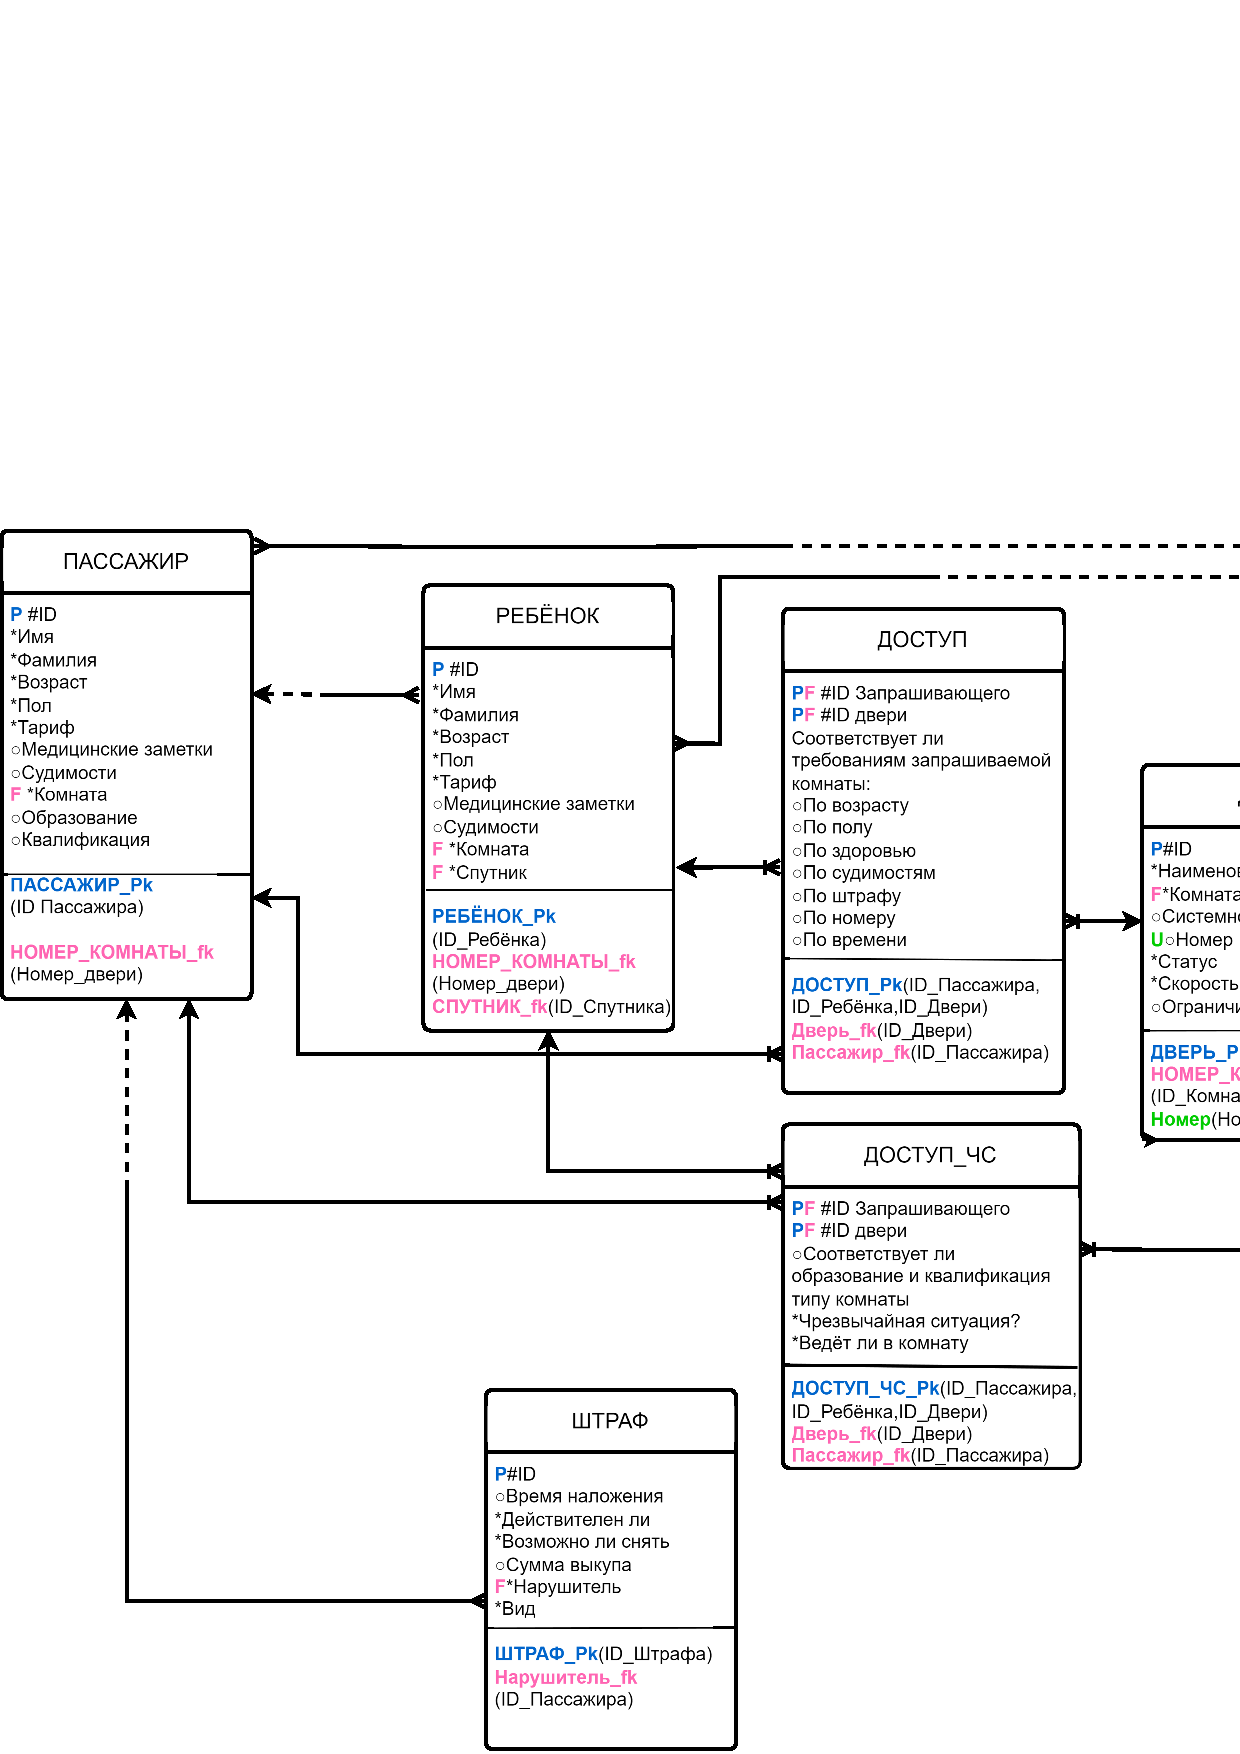
\includegraphics[width=1\linewidth]{images/CommonScheme3}
	\caption{Реляционная модель данных}
	\label{fig:commonscheme3}
\end{figure}

\subsubsection{Требования к безопасности}
1. Поддержка современных операционных систем, обеспечивающих стабильную и безопасную работу на различных платформах;

2. Реализация защиты от атак типа SQL-инъекций, предотвращающей нежелательное вмешательство в работу приложения;

3. Регулярное обновление компонентов системы для предотвращения уязвимостей, связанных с устаревшим программным обеспечением.

\subsubsection{Требования к программному обеспечению}

Для реализации программной системы необходимо подготовить следующие компоненты:

Интерпретатор языка программирования Python; 

СУБД SQLite;

Для работы и приложения требуется ОС Windows 7 или более поздняя версия/Ubuntu 16.0 или более поздняя версия с установленным интерпретатором языка python и установленной СУБД SQLite.

\subsubsection{Требования к аппаратному обеспечению}
Системе необходим центральный процессор с количеством ядер от 2 и выше с частотой ядра от 1.4 ГГц. Объем оперативной памяти – 4 Гб.
Свободное место на диске: 13МБ

\subsection{Требования к оформлению документации}

Требования к стадиям разработки программ и программной документации для вычислительных машин, комплексов и систем независимо от их
назначения и области применения, этапам и содержанию работ устанавливаются ГОСТ 19.102–77. Программная документация должна включать в себя:

1. Анализ предметной области;

2. Техническое задание;

3. Технический проект;

4. Рабочий проект.


\section{Технический проект}
\subsection{Общая характеристика организации решения задачи}

Необходимо спроектировать и разработать приложение, которое обеспечит функционирование СКУД на круизном лайнере AIDABlu.

Приложение представляет собой панель управления для работы с данными в базе данных системы. Панель содержит текстовую и графическую информацию (TreeView).

Приложение является десктопным, т.е. располагается и запускается внутри лишь одной операционной системы. Каждое окно приложения (за исключением главного) – это панель управления для конкретной таблицы базы данных. Приложение разработано на языке Python v3.10. Управление данными БД реализовано с помощью библиотеки sqlite3 и SQL -- языка структурированных запросов к базе данных.

\subsection{Общие сведения о программно-информационной системе}

Полное наименование системы: Программное обеспечение для системы контроля и управления доступом на круизном судне.

Краткое обозначение системы: \textquotedbl СКУД на круизном лайнере \textquotedbl.

Описание системы: \textquotedbl СКУД на круизном лайнере \textquotedbl предназначена для корпораций, организующих круизные путешествия, предоставляя им платформу для удобного контроля и управления данными всей бизнес-системы круизного лайнера на время поездки. Система создана для обеспечения комфортной и безопасной поездки каждого пассажира и функционирования в форс-мажорных ситуациях.

Условия эксплуатации: \textquotedbl СКУД на круизном лайнере \textquotedbl предназначена для использования как в нормальных, так и в чрезвычайных условиях работы.

Архитектура системы: Программное обеспечение основано на десктопной архитектуре, используя современные технологии разработки, включая TKinter и CustomTkinter для Front-End части и sqlite3 для реализации запросов к БД в Back-End. Система использует базу данных SQLite.

Технологии и инструменты: В разработке использовались tkinter, customtkinter, sqlite3, asyncio, time

\subsection{Обоснование выбора технологии проектирования}

\subsubsection{Описание используемых технологий и языков программирования}

В процессе разработки приложения используются программные средства и языки программирования. Каждое программное средство и каждый язык программирования применяется для круга задач, при решении которых они необходимы.

\subsubsection {tkinter}
Выбор tkinter для Front-End обосновывается его простотой и кроссплатформенной поддержкой, а также минимальными требованиями к интерфейсу в пользу быстродействия. 

Пакет tkinter («интерфейс Tk») - это интерфейс Python для создания GUI. Tkinter доступен на большинстве платформ Unix, включая macOS, а также на системах Windows.

Tkinter входит в состав большинства инсталляций Python, что делает его легкодоступным для разработчиков, которые хотят создавать приложения с графическим интерфейсом, не требуя дополнительных инсталляций или библиотек.

\subsubsection {customtkinter}
Выбор customtkinter для Front-End обосновывается его расширенным функционалом по сравнению с tkinter. Customtkinter предлагает большой список параметров для настройки виджетов и является полностью совместимым с элементами tkinter.

CustomTkinter - это библиотека пользовательского интерфейса для настольных компьютеров на основе Tkinter, которая обеспечивает современный вид и полностью настраиваемые виджеты.

\subsubsection {SQLite}
Выбор SQLite в качестве системы управления базами данных также обосновывается его удобством как на этапе проектирования, так и на этапе реализации.

SQLite - это библиотека на языке C, которая предоставляет легкую дисковую базу данных, не требующую отдельного серверного процесса и позволяющую обращаться к базе данных с помощью нестандартного варианта языка запросов SQL. Некоторые приложения могут использовать SQLite для внутреннего хранения данных. Также можно создать прототип приложения с использованием SQLite, а затем перенести код на более крупную базу данных, такую как PostgreSQL или Oracle.

\subsubsection {asyncio и time}
Модули asyncio и time были использованы для актуализации работы системы в реальном времени и многопоточном режиме.


\subsubsection{Язык структурированных запросов к базе данных SQL}
SQL - это стандартизированный язык программирования, который используется для управления реляционными базами данных и выполнения различных операций над данными в них. 

SQL используется для следующего:
\begin{itemize}
	\item изменение структуры таблиц данных и индексов базы данных;
	\item добавление, обновление и удаление строк данных;
	\item извлечение подмножеств информации из реляционных систем управления базами данных (РСУБД).
\end{itemize}


\subsubsection{Язык программирования Python}

\paragraph{Достоинства языка Python}
Python - очень продуктивный язык. Благодаря простоте Python разработчики могут сосредоточиться на решении проблемы. Написание кода экономит время и освобождает его для более ёмкой работы с другими составляющими проекта.

Python поставляется под лицензией OSI с открытым исходным кодом. Это делает его свободным для использования и распространения. Можно загружать исходный код, изменять его и даже распространять свою версию Python. Это полезно для организаций, которые хотят изменить некоторые специфические функции и использовать свою версию для разработки.

Стандартная библиотека Python огромна, в ней можно найти практически все функции, необходимые для решения любой задачи. Таким образом, не придется зависеть от внешних библиотек.

Во многих языках, таких как C/C++, для запуска программы на разных платформах необходимо изменять код. С Python дело обстоит иначе. Вы пишете один раз и запускаете программу в любом месте.

\paragraph{Недостатки языка Python}

Язык программирования Python использует большой объем памяти. Это может быть недостатком при создании приложений, когда предпочтение отдаётся оптимизации памяти.

Python используется для программирования на стороне сервера. Пользователь не видит Python на стороне клиента или в мобильных приложениях.

Python - динамически типизированный язык, поэтому тип данных переменной может измениться в любой момент. Переменная, содержащая целое число, в будущем может стать строкой, что может привести к ошибкам времени выполнения.

\subsection{Проектирование пользовательского интерфейса}
На основании требований к пользовательскому интерфейсу, представленных в пункте 2.3 технического задания, был разработан графический интерфейс десктопного приложения с применением python tkinter, customtkinter и SQLite. Этот процесс подчеркивает важность интуитивно понятного и эффективного взаимодействия с пользователем. Разработанный интерфейс ориентирован на обеспечение легкости в использовании и интуитивного понимания функционала приложения, предоставляя пользователю простое и эффективное взаимодействие с приложением.

1. \textbf{Навигация по таблицам с данными:} Реализация функции навигации на основе полей psr\underline{ }btn, psr\underline{ }ua\underline{ }btn, drs\underline{ }btn, rms\underline{ }btn, pns\underline{ }btn, acs\underline{ }btn;

2. \textbf {Панель управления для каждой из таблиц с данными:} диверсификация интерфейсов происходит на основе метода show\underline{ }table класса Controller;

3. \textbf{Отображение текущей таблицы с данными в реальном времени:} актуальность этого графического элемента (дерева) поддерживается за счёт методов TreeRefresh и TreeCreate класса Controller;

4. \textbf{Воздействие на внесённые данные базы:} Добавление, изменение или удаление элементов реализованы в методах add\underline{ }element, update\underline{ }element и delete\underline{ }element класса Tables соответственно, внутри которых формирование строк запросов к БД реализовано с помощью класса Utils.

5. \textbf{Навигация и лёгкий поиск среди элементов среди данных:} Пользователь может переходить по элементам последовательно (метод MoveTo класса Controller), или же использовать отдельное текстовое поле для метода search\underline{ }element класса Tables, перейдя сразу к искомому элементу таблицы.

6. \textbf{Отображение локального времени:} Учитывая специфику проекта -- систему для круизного лайнера, учтено, что часовой пояс может измениться во время путешествия. На уровне python и SQL была установлена привязка к локальному времени (localtime), а функционал часов запущен в асинхронном потоке во избежание ошибок и помех работы основной системы.

7. \textbf{Запрос доступа к двери:} На основе правил, прописанных в полях Комнаты, к которой привязана выбранная Дверь, в отдельном окне отображается информация о том, есть ли у Пассажира доступ к этой Двери.

\begin{figure} [ht]
	\centering
	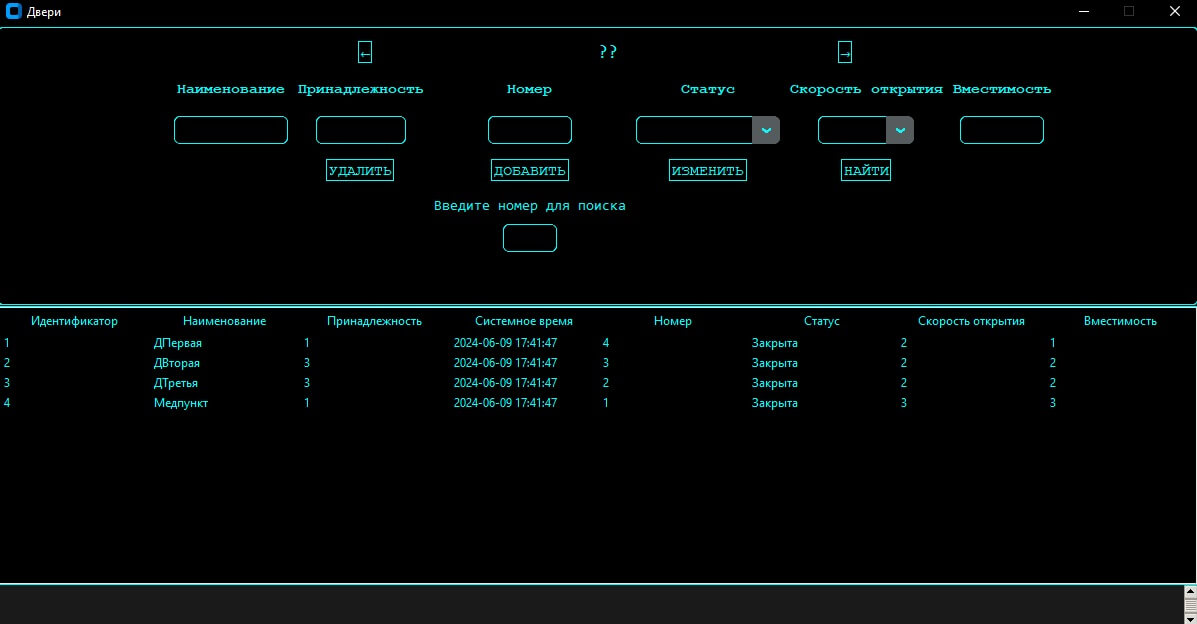
\includegraphics[width=1\linewidth]{images/Example2}
	\caption{Модели интерфейса <<Панель управления для каждой из таблиц с данными>> и <<Отображение текущей таблицы с данными в реальном времени>>}
	\label{fig:example2}
\end{figure}

Процесс изменения данных максимально упрощён и включает следующие шаги:

1. В главном меню пользователь выбирает поле с названием необходимого ему вида данных.

2. В появившемся окне пользователь находит нужный ему элемент посредством <<Пролистывания>> или посредством поиска по идентификатору, при нажатии на соответствующие подписанные поля.

3. Пользователь изменяет некоторые данные в полях элемента и выбирает опцию <<Изменить>>, если ему нужно было редактировать элемент, или <<Удалить>>, если была необходимость удалить элемент.

4. Если пользователю необходимо добавить элемент, он должен заполнить поля ввода: Наименование, принадлежность, номер, статус, скорость открытия, вместимость (В случае работы с данными о дверях) и выбрать опцию <<Добавить>>.

5. На последнем этапе, если все обязательные поля были заполнены данными корректного формата, пользователь получает сообщение об успешном проведении операции и она выполняется.

\begin{figure} [ht]
	\centering
	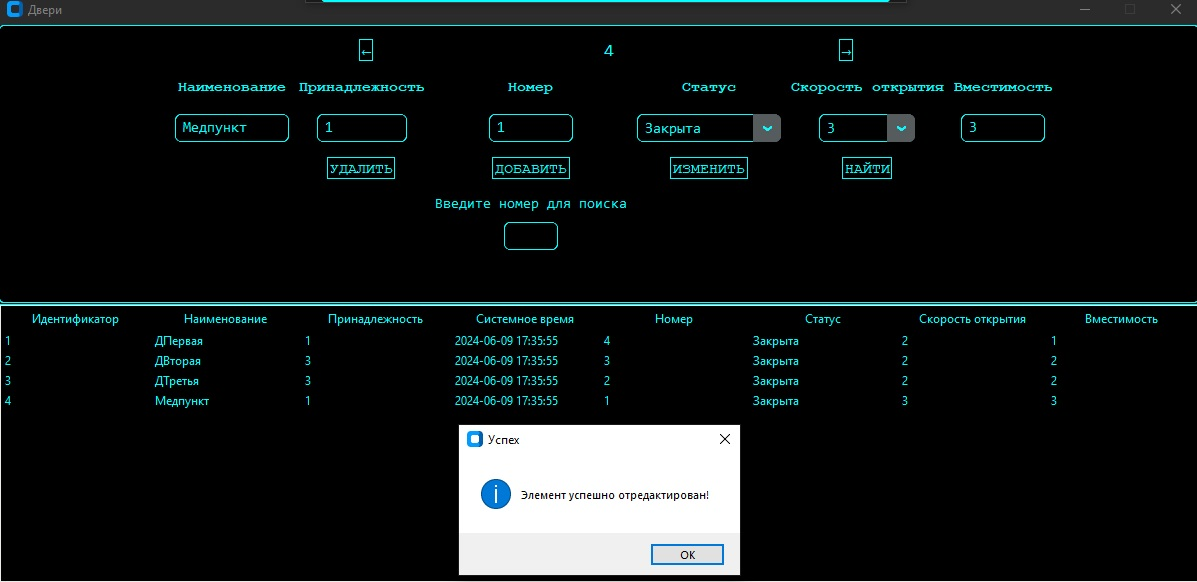
\includegraphics[width=1\linewidth]{images/Example1}
	\caption{Модель интерфейса <<Изменение данных элемента>>}
	\label{fig:example1}
\end{figure}
Процесс получения информации о доступе является еще более простым и состоит из следующих этапов:

1. В главном меню пользователь выбирает опцию <<Проверка доступа>>.

2. В появившемся окне пользователь с помощью переключателя выбирает нужную ему группу поиска среди пассажиров - таблицу <<Пассажиры>> или <<Дети>>.

3. Пользователь вводит идентификаторы пассажира и двери в поля \textquotedbl Пассажир \textquotedbl и \textquotedbl Дверь \textquotedbl соответственно и выбирает опцию <<Проверить доступ>>

4. На последнем этапе, если все обязательные поля были заполнены данными корректного формата и в БД содержатся данные о предоставленном/отказанном доступе, пользователь получает сообщение о том, есть ли у указанного пассажира доступ к указанной двери.

\begin{figure} [ht]
	\centering
	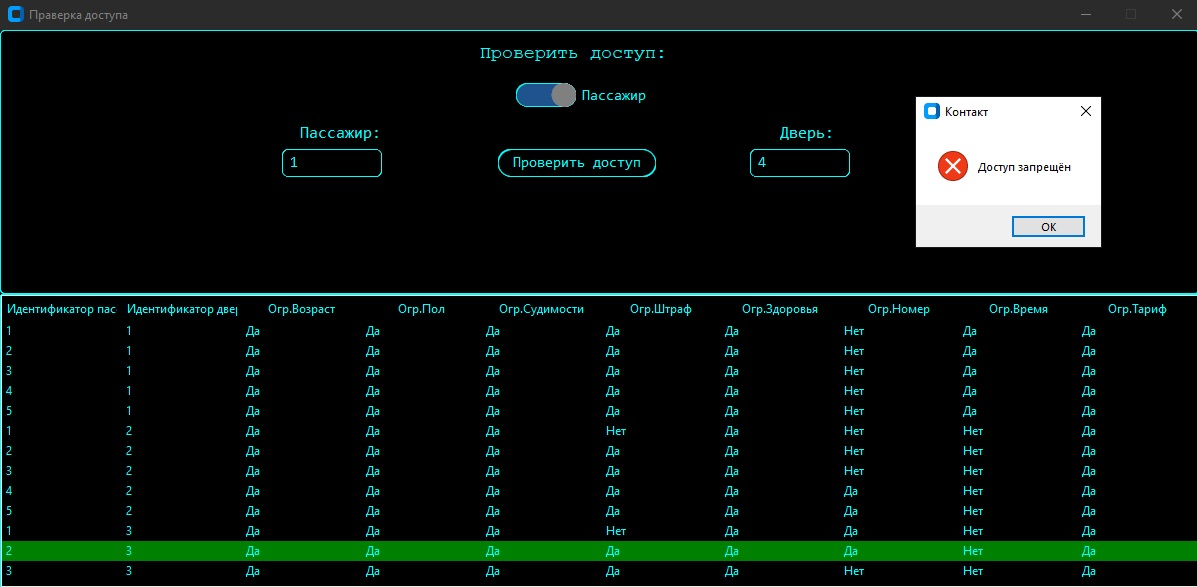
\includegraphics[width=1\linewidth]{images/Example3}
	\caption{Модель интерфейса <<запрос доступа к двери>>.}
	\label{fig:example3}
\end{figure}


\subsection{Диаграмма размещения}
Диаграмма размещения, отображаемая на рисунке \ref{fig:commonscheme4}, является фундаментальным инструментом для иллюстрации взаимосвязей между программными и аппаратными компонентами системы. Этот элемент визуализации служит для акцентирования значимости стратегического планирования
в процессе разработки распределенных систем. Детальное и глубокое понимание этих взаимосвязей критически важно для успешного создания и функционирования распределенных информационных систем.

Каждый компонент системы, будь то программный или аппаратный, играет важную роль в обеспечении её общей эффективности и надежности.
Подход, основанный на стратегическом планировании, способствует оптимизации этих взаимодействий и повышает вероятность успешной реализации и эксплуатации системы в целом.

\begin{figure} [ht]
	\centering
	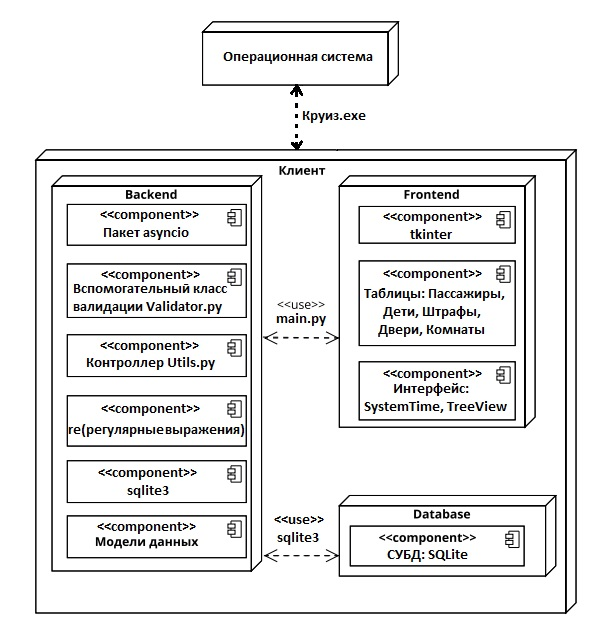
\includegraphics[width=1\linewidth]{images/CommonScheme4}
	\caption{Диаграмма размещения}
	\label{fig:commonscheme4}
\end{figure}
Она является хорошим средством для показа маршрутов перемещения объектов и компонентов в распределенной системе.

\subsection{Описание архитектуры приложения}

Архитектура приложения, реализованная в рамках текущей работы, базируется на модели MVC (Model-View-Controller). Этот паттерн был избран из-за его способности к эффективному распределению функциональных обязанностей между структурными компонентами системы, а также способствованию упрощению процессов разработки и тестирования.

MVC реализован следующим образом:

1. Модель (Model) и Контроллер (Controller): Эти компоненты обеспечивают управление бизнес-логикой и обработку данных, а также связь между пользовательским интерфейсом и базой данных;

2. Представление (View): Реализовано через фронтенд, использующий пакеты tkinter, customtkinter и treeview, и отвечающий за визуализацию информации и интерактивное взаимодействие с пользователем.

Ключевым аспектом в управлении данными является использование системы управления базами данных SQLite. Этот выбор был обусловлен высокой надежностью SQLite, её устойчивостью к атакам типа \textquotedbl SQL-Инъекция \textquotedbl и гибкостью в обработке сложных запросов, что имеет критическое значение для эффективного функционирования бэкенда.

Применение архитектуры MVC принесло следующие ключевые преимущества:

\begin{itemize}
	\item Четкое Разделение Обязанностей: Эффективное разграничение между пользовательским интерфейсом (класс main.py и controller.py) и back-end логикой (tables.py) значительно упрощает процесс разработки и последующей поддержки системы
	\item Гибкость и Масштабируемость: Благодаря MVC, архитектура приложения легко адаптируется и масштабируется, что позволяет разработчикам
	модифицировать или расширять отдельные части системы без влияния на другие;
	\item Упрощение Тестирования: Независимость компонентов архитектуры MVC облегчает процедуру тестирования, позволяя проводить её для каждого элемента в отдельности
\end{itemize}

Такой подход устанавливает предпочтительную форму записи организации функционала и способ его использования в тестировании. Он обеспечивает создание надежной, гибкой и масштабируемой системы, а также применим как в крупных, так и в малых проектах.

Модули:

В backend применяется модуль asyncio для организации работы системного времени в отдельном потоке.

Модуль re включается для работы с регулярными выражениями для задания правил написания, валидации полей.

Модуль sqlite3 используется для организации подключения и запросов к базе данных.

Для создания frontend используются модули tkinter, customtkinter и treeView. TreeView необходим для отображения виджета древа таблицы в реальном времени,  customtkinter - для основного интерфейса приложения, а tkinter - для служебного упорядочивания элементов интерфейса customtkinter и treeview.

Классы:

main.py - в этом классе прописан front-end главного меню с последующей передачей вводимых данных в другие компоненты.

Utils.py - служебный класс, внутри которого реализованы функции запросов к базе данных, асинхронное обновление системного времени(Например, подключение к БД - create\underline{ }connection(), чтение - read\underline{ }single\underline{ }row(), запрос - execute\underline{ }query() и т.д.).

Validator.py - служебный класс для задания правил написания (валидации). Необходим для проверки корректности вводимых данных(Например, метод FKValid() - для валидации внешних ключей, overvalidation() для дополнительной проверки корректности перед валидацией)

Controller.py - в этом классе прописана front-end логика панели управления таблицами данных с последующей передачей вводимых данных в другие компоненты, а также выводом полученных данных на экран.

Tables.py - служебный класс, созданный для формирования запросов к БД. Вся логика взаимодействия с данными внутри базы, таким как добавление - add\underline{ }element(), удаление - delete\underline{ }element() и т.д., содержится в этом классе.
\ifПрактика{}\else{
   \section{Рабочий проект}
\subsection{Описание классов системы}
Система реализована с помощью следующих программных классов:

\begin{itemize}
	\item \textquotedbl main \textquotedbl является фундаментальным классом для главного меню. Помимо основных свойств, таких как connection, экземпляров utils, controller и tables, содержит в себе стартовые виджеты;
	\item \textquotedbl Controller \textquotedbl -- расширяет \textquotedbl main \textquotedbl, представляя панель управления таблицами, необходимую для взаимодействия пользователя с данными внутри таблицы;
	\item \textquotedbl Utils \textquotedbl применяется для отправки запросов в БД. Содержит только самые необходимые методы, взаимодействующие с БД непосредственно;
	\item \textquotedbl Tables \textquotedbl служит для формирования необходимых сложных запросов к БД. Сформировав строку, класс использует \textquotedbl Utils \textquotedbl для отправки;
	\item \textquotedbl Validator \textquotedbl представляет собой служебный класс, конфигурирующий интерфейс таким образом, чтобы пользователь не мог ввести данные неподходящего формата.
\end{itemize}

Описание полей и методов программных классов приведено в таблицах \ref{class:table1}-\ref{class:table5}.

\renewcommand{\arraystretch}{0.8} % уменьшение расстояний до сетки таблицы
\begin{xltabular}{\textwidth}{|X|p{2.5cm}|>{\setlength{\baselineskip}{0.7\baselineskip}}p{4.85cm}|>{\setlength{\baselineskip}{0.7\baselineskip}}p{4.85cm}|}
\caption{Описание класса main\label{class:table1}}\\
\hline \centrow \setlength{\baselineskip}{0.7\baselineskip} Название класса & \centrow \setlength{\baselineskip}{0.7\baselineskip} Модуль, к которому относится класс & \centrow Описание поля/метода & \centrow Поле/метод \\
\hline \centrow 1 & \centrow 2 & \centrow 3 & \centrow 4\\ \hline
\endfirsthead
\caption*{Продолжение таблицы \ref{class:table1}}\\
\hline \centrow 1 & \centrow 2 & \centrow 3 & \centrow 4\\ \hline
\finishhead
main & Главный модуль & isES -- поле для определения режима работы программы (Обычный или ЧС) & bool isES\\
\hline  & Главный модуль & window -- экземпляр класса customtkinter.CTk(), представляющий окно & CTk window\\
\hline  & Главный модуль & frame -- экземпляр класса customtkinter.CTkFrame(), представляющий поле для виджетов & CTkFrame frame\\
\hline  & Главный модуль & connection -- строка, содержащая путь для подключения к БД & string connection\\
\hline  & Главный модуль & ask\underline{ }lb, timer\underline{ }lb -- виджеты текста в главном меню &
CTkLabel ask\underline{ }lb

CTkLabel timer\underline{ }lb
\\
\hline  & Главный модуль & pns\underline{ }btn, rms\underline{ }btn, drs\underline{ }btn, psr\underline{ }btn, psr\underline{ }ua\underline{ }btn -- виджеты кнопок в главном меню &
CTkButton pns\underline{ }btn

CTkButton rms\underline{ }btn

CTkButton drs\underline{ }btn

CTkButton psr\underline{ }btn

CTkButton psr\underline{ }ua\underline{ }btn
\\
\hline  & Главный модуль & on\underline{ }closing -- метод для вывода вопроса о том, уверен ли пользователь в своём решении выйти & on\underline{ }closing() Возвращает: ничего\\ 
\end{xltabular}
\renewcommand{\arraystretch}{1.0} % восстановление сетки
 
\begin{xltabular}{\textwidth}{|X|p{2.5cm}|>{\setlength{\baselineskip}{0.7\baselineskip}}p{4.85cm}|>{\setlength{\baselineskip}{0.7\baselineskip}}p{4.85cm}|}
	\caption{Описание класса Controller \label{class:table2}}\\
	\hline \centrow \setlength{\baselineskip}{0.7\baselineskip} Название класса & \centrow \setlength{\baselineskip}{0.7\baselineskip} Модуль, к которому относится класс & \centrow Описание поля/метода & \centrow Поле/метод \\
	\hline \centrow 1 & \centrow 2 & \centrow 3 & \centrow 4\\ \hline
	\endfirsthead
	\caption*{Продолжение таблицы \ref{class:table2}}\\
	\hline \centrow 1 & \centrow 2 & \centrow 3 & \centrow 4\\ \hline
	\finishhead
Controller & Главный модуль & styles\underline{ }init -- метод для инициализации стилей и добавления его в список ttk.element\underline{ }names & styles\underline{ }init(st). Принимает на вход экземпляр класса Style, который будет настраивать. 

Возвращает: ничего\\
\hline  & Главный модуль & show\underline{ }table -- метод для перехода к панели управления выбранной таблицей. Отображает, настраивает и группирует каждый элемент по сетке & show\underline{ }table(which, window, tables, connection). 

Принимает на вход название таблицы, экземпляр окна, экземпляр tables, и строку подключения connection. 

Возвращает: ничего\\
\hline  & Главный модуль & fields\underline{ }creation -- метод, вызываемый в show\underline{ }table и дополняющий его. Определяет и направленно настраивает поля ввода информации & fields\underline{ }creation(which, frameEx, window). 

На вход принимает название таблицы, экземпляр поля для виджетов, экземпляр окна.

Возвращает: tuple (validatedTFs, combolist) -- кортеж сформированных полей ввода\\
\hline  & Главный модуль & clear -- метод, очищающий поля ввода & clear(keyLabel, combinedControls, window). 

На вход принимает таблицу отображения Id текущей строки для очищения, кортеж полей ввода, экземпляр окна. 

Возвращает: ничего\\
\hline  & Главный модуль & TreeCreate -- метод, отображающий текущую таблицу в виде виджета древа & TreeCreate(tree, table, tableWin, connection). 

На вход принимает экземпляр класса ttk.TreeView, который будет пересоздавать, название таблицы, экземпляр поля виджетов, строку подключения. 

Возвращает: TreeView.tree -- созданный виджет древа\\
\hline  & Главный модуль & TreeRefresh -- метод, обновляющий виджет древа & TreeRefresh(tree, table, connection). 

На вход принимает экземпляр класса ttk.TreeView, который будет обновлять, название таблицы, строку подключения. 

Возвращает: Ничего\\
\hline  & Главный модуль & MoveTo -- метод для перехода просмотра к конкретному элементу таблицы по индентификатору & MoveTo(id, table, combinedControls, currentLb, window, connection). 

На вход принимает идентификатор элемента для перехода, имя таблицы, кортеж полей вывода, табличку отображения текущего Id, экземпляр окна и строку подключения. 

Возвращает: Ничего\\
\hline  & Главный модуль & show\underline{ }acc -- метод для перехода к окну проверки доступа & show\underline{ }acc(connection, isES, tables, window). 

На вход принимает строку подключения к БД, флаг ЧС, экземпляр класса tables, экземпляр окна. 

Возвращает: Ничего\\
\hline  & Главный модуль & toggle\underline{ }ES -- метод обработки состояний переключателя, применяемый в определении одной из двух таблиц для показа & toggle\underline{ }ES(switch, psrlb, tables,connection, tree, isES). 

На вход принимает экземпляр переключателя, текстовое поле для изменения выводимой информации, строку подключения, экземпляр виджета древа и флаг ЧС.

\end{xltabular}

\renewcommand{\arraystretch}{1.0} % восстановление сетки

\begin{xltabular}{\textwidth}{|X|p{2.5cm}|>{\setlength{\baselineskip}{0.7\baselineskip}}p{4.85cm}|>{\setlength{\baselineskip}{0.7\baselineskip}}p{4.85cm}|}
	\caption{Описание класса Utils \label{class:table3}}\\
	\hline \centrow \setlength{\baselineskip}{0.7\baselineskip} Название класса & \centrow \setlength{\baselineskip}{0.7\baselineskip} Модуль, к которому относится класс & \centrow Описание поля/метода & \centrow Поле/метод \\
	\hline \centrow 1 & \centrow 2 & \centrow 3 & \centrow 4\\ \hline
	\endfirsthead
	\caption*{Продолжение таблицы \ref{class:table3}}\\
	\hline \centrow 1 & \centrow 2 & \centrow 3 & \centrow 4\\ \hline
	\finishhead
Utils & Главный модуль & create\underline{ }connection -- метод создаёт подключение к базе данных & create\underline{ }connection(path). 

На вход принимает строковый путь к файлу базы данных. 

Возвращает: sqlite3.connection connection - экземпляр созданного подключения\\
\hline  & Главный модуль & read\underline{ }single\underline{ }row -- считывает единственную строку с БД & read\underline{ }single\underline{ }row(id, connection, table). 

На вход принимает идентификатор, по которому будет считываться строка, экземпляр подключения, название таблицы 

Возвращает: строку в формате кортежа\\
\hline  & Главный модуль & execute\underline{ }query -- посылает команду в БД & execute\underline{ }query(
connection, query).

На вход принимает экземпляр подключения и строку команды для выполнения.

Возвращает: bool True/bool False -- флаг о том, успешно ли выполнен запрос\\
\hline  & Главный модуль & execute\underline{ }read\underline{ }query -- отдельный метод для послания запроса в БД на чтение & execute\underline{ }read\underline{ }query(
connection, query).

На вход принимает экземпляр подключения и строку команды для выполнения.

Возвращает: строку в формате кортежа\\
\hline  & Главный модуль & timetick -- асинхронный метод для отображения и вывода текущего времени в главном меню & timetick(timerLb).

На вход принимает, куда будет выводиться время.

Возвращает: ничего\\
\hline  & Главный модуль & asyncMLoop -- метод для обеспечения асинхронной работы окна с часами & asyncMLoop(wndw).

На вход принимает окно главного меню.

Возвращает: ничего\\
\hline  & Главный модуль & asyncStart -- асинхронный метод для настройки взаимодействия главного меню с часами в асинхронном порядке и обновления полей со временем в БД & asyncStart(window, timer\underline{ }lb, connection).

На вход принимает экземпляр окна, поле для вывода времени, строку подключения к БД.

Возвращает: Ничего\\
	
\end{xltabular}
\renewcommand{\arraystretch}{1.0} % восстановление сетки

\begin{xltabular}{\textwidth}{|X|p{2.5cm}|>{\setlength{\baselineskip}{0.7\baselineskip}}p{4.85cm}|>{\setlength{\baselineskip}{0.7\baselineskip}}p{4.85cm}|}
	\caption{Описание класса Tables \label{class:table4}}\\
	\hline \centrow \setlength{\baselineskip}{0.7\baselineskip} Название класса & \centrow \setlength{\baselineskip}{0.7\baselineskip} Модуль, к которому относится класс & \centrow Описание поля/метода & \centrow Поле/метод \\
	\hline \centrow 1 & \centrow 2 & \centrow 3 & \centrow 4\\ \hline
	\endfirsthead
	\caption*{Продолжение таблицы \ref{class:table4}}\\
	\hline \centrow 1 & \centrow 2 & \centrow 3 & \centrow 4\\ \hline
	\finishhead
	Tables & Главный модуль & self\underline{ }definition -- метод переводит названия таблиц данных с русского языка на английский для последующих запросов к БД & self\underline{ }definition(which). 
	
	На вход принимает строку названия на русском языке. 
	
	Возвращает: строку названия на английском языке\\
	\hline  & Главный модуль & timeAppend -- метод, переводящий строку времени из формата <<ЧЧММСС>> в формат <<ЧЧ:ММ:СС>> & timeAppend(timeString). 
	
	На вход принимает неотформатированную строку времени. 
	
	Возвращает: строку времени в отформатированном виде\\
	\hline  & Главный модуль & penalty\underline{ }check -- метод, сравнивающий данные о штрафных ограничениях данных о Дверях и данных о Штрафах & penalty\underline{ }check(pennies, type). 
	
	На вход принимает кортеж из найденных по принадлежности штрафов и строку типа штрафа, с которой нужно сопоставить элементы кортежа. 
	
	Возвращает: флаг о том, совпали ли типы\\
	\hline  & Главный модуль & check\underline{ }access -- метод реализации опции <<Проверка доступа>>, проверяет введённые данные на наличие в базе и выводит информацию о предоставлении доступа. & check\underline{ }access(psr\underline{ }Tf, dor\underline{ }Tf, switch, connection). 
	
	На вход принимает экземпляры текстовых полей куда были введены идентификаторы для поиска, жкземпляр переключателя, строку подключения к БД. 
	
	Возвращает: ничего\\
	\hline  & Главный модуль & start\underline{ }accesses -- метод заполнения данных о доступе пассажиров к дверям по каждому из критериев ограничений. & start\underline{ }accesses(
	connection, psr\underline{ }switch). 
	
	На вход принимает строку подключения к БД и экземпляр переключателя. 
	
	Возвращает: ничего\\
	\hline  & Главный модуль & add\underline{ }element -- метод, реализующий опцию формирования запроса добавления элемента в БД. & add\underline{ }element(table, combinedControls, currentLb, tree, tableWin, connection, window). 
	
	На вход принимает строку названия таблицы, кортеж полей ввода, экземпляр текстового поля для отображения идентификатора текущего элемента, экземпляр виджета древа, экземпляр контейнера для виджетов, строку подключения, экземпляр окна. 
	
	Возвращает: ничего\\
	\hline  & Главный модуль & delete\underline{ }element -- метод, реализующий опцию формирования запроса удаления элемента в БД. & delete\underline{ }element(table, key, currentLb, combinedControls, tree, connection, window). 
	
	На вход принимает строку названия таблицы, идентификатор текущего элемента, кортеж полей ввода, экземпляр текстового поля для отображения идентификатора текущего элемента, экземпляр виджета древа, строку подключения, экземпляр окна. 
	
	Возвращает: ничего\\
	\hline  & Главный модуль & update\underline{ }element -- метод, реализующий опцию формирования запроса изменения элемента в БД. & update\underline{ }element(table, combinedControls, key, tree, connection). 
	
	На вход принимает строку названия таблицы, кортеж полей ввода,  идентификатор текущего элемента, экземпляр виджета древа, строку подключения.
	
	Возвращает: ничего\\
	\hline  & Главный модуль & search\underline{ }element -- метод, реализующий опцию поиска элемента в БД. & search\underline{ }element(
	combinedControls, table, tf, currentLb, connection, window). 
	
	На вход принимает кортеж полей ввода, строку названия таблицы, текстовое поля для воода идентификатора поиска, экземпляр текстового поля для отображения идентификатора текущего элемента,  строку подключения.
	
	Возвращает: ничего\\
	\hline  & Главный модуль & list\underline{ }table -- метод, реализующий опцию \textquotedbl пролистывания \textquotedbl текущей таблицы данных. & list\underline{ }table(direction, table, connection, window). 
	
	На вход принимает флаг направления (вперёд или назад), строку названия таблицы, строку подключения к БД, экземпляр окна.
	
	Возвращает: массив данных текущего элемента\\
	\hline  & Главный модуль & configure\underline{ }list -- метод, дополняющий list\underline{ }table и выводящий данные текущего элемента в поля ввода . & configure\underline{ }list(direction, table, combinedControls, currentLb, connection, window). 
	
	На вход принимает флаг направления (вперёд или назад), строку названия таблицы, кортеж полей ввода, экземпляр текстового поля для отображения идентификатора текущего элемента, строку подключения к БД, экземпляр окна.
	
	Возвращает: массив данных текущего элемента\\
	
\end{xltabular}
\renewcommand{\arraystretch}{1.0} % восстановление сетки


\begin{xltabular}{\textwidth}{|X|p{2.5cm}|>{\setlength{\baselineskip}{0.7\baselineskip}}p{4.85cm}|>{\setlength{\baselineskip}{0.7\baselineskip}}p{4.85cm}|}
	\caption{Описание класса Validator \label{class:table5}}\\
	\hline \centrow \setlength{\baselineskip}{0.7\baselineskip} Название класса & \centrow \setlength{\baselineskip}{0.7\baselineskip} Модуль, к которому относится класс & \centrow Описание поля/метода & \centrow Поле/метод \\
	\hline \centrow 1 & \centrow 2 & \centrow 3 & \centrow 4\\ \hline
	\endfirsthead
	\caption*{Продолжение таблицы \ref{class:table5}}\\
	\hline \centrow 1 & \centrow 2 & \centrow 3 & \centrow 4\\ \hline
	\finishhead
	Validator & Главный модуль & connection -- строка для подключения к базе данных & string connection\\
	\hline  & Главный модуль & validation\underline{ }digits -- метод, использующийся для регистрации правила валидации цифр & validation\underline{ }digits(
	stringVal). 
	
	На вход принимает строку для проверки соответствия правилу.
	
	Возвращает: ту часть строки, что соответствует маске цифр\\
	\hline  & Главный модуль & validation\underline{ }text -- метод, использующийся для регистрации правила валидации символов Кириллицы & validation\underline{ }text(
	stringVal). 
	
	На вход принимает строку для проверки соответствия правилу.
	
	Возвращает: ту часть строки, что соответствует маске символов Кириллицы\\
	\hline  & Главный модуль & validation\underline{ }char -- метод, использующийся для регистрации правила валидации единичного символа Кириллицы & validation\underline{ }char(
	stringVal). 
	
	На вход принимает строку для проверки соответствия правилу.
	
	Возвращает: ту часть строки, что соответствует маске единичного символа Кириллицы\\
	\hline  & Главный модуль & validation\underline{ }time -- метод, использующийся для регистрации правила валидации текстового поля для ввода времени & validation\underline{ }time(
	stringVal). 
	
	На вход принимает строку для проверки соответствия правилу.
	
	Возвращает: ту часть строки, что соответствует маске формата времени\\
	\hline  & Главный модуль & FKValid -- метод, проверяющий наличие элемента с идентификатором для создания внешнего ключа & FKValid(number, tableName). 
	
	На вход принимает номер для поиска, строку названия таблицы.
	
	Возвращает: флаг о том, был ли найден элемент\\
	\hline  & Главный модуль & validate\underline{ }single -- метод, задающий правила ввода для единичного поля ввода & validate\underline{ }single(element, window, type). 
	
	На вход принимает экземпляр поля ввода, экземпляр окна, строку типа валидации.
	
	Возвращает: поле ввода с изменёнными правилами\\
	\hline  & Главный модуль & validate\underline{ }whole -- метод, задающий правила ввода для массива полей ввода & validate\underline{ }whole(tfS, which, window). 
	
	На вход принимает массив полей ввода, строку названия таблицы данных, экземпляр окна.
	
	Возвращает: массив полей ввода с изменёнными правилами\\
	\hline  & Главный модуль & overvalidation -- метод, проверяющий уже введённые данные на корректность перед отправкой & overvalidation(table, combinedControls). 
	
	На вход принимает строку названия таблицы, кортеж полей ввода.
	
	Возвращает: флаг соответствия корректности\\
	
\end{xltabular}
\renewcommand{\arraystretch}{1.0} % восстановление сетки
\subsection{Модульное тестирование программной системы}
\subsubsection{Структура тестового проекта}

В рамках тестирования программного обеспечения была разработан тестовый проект, структура которого представлена на рисунке~\ref{fig:test1}. Данный проект включает в себя модульные тесты для различных компонентов системы.
Тестирование моделей и контроллеров позволяет обеспечить надежность и корректность работы программного обеспечения. 
\begin{figure}[H]
	\centering
	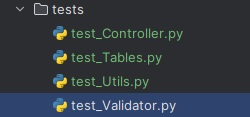
\includegraphics[width=0.6\linewidth]{images/test1}
	\caption{Структура тестового проекта}
	\label{fig:test1}
\end{figure}
Тестовый проект включает в себя следующие ключевые элементы:
\begin{itemize}
	\item test\underline{ }Controller.py: Наборы модульных тестов для класса панели управления Controller;
	\item test\underline{ }Tables.py: Наборы модульных тестов для класса формирования запросов к БД Tables;
	\item test\underline{ }Validator.py: Наборы модульных тестов для вспомогательного класса валидации Validator;
	\item test\underline{ }Utils.py: Наборы модульных тестов для cлужебного класса запросов в БД.
\end{itemize}
Модульные тесты для класса Tables.py, который является основным классом для формирования запросов в БД, позволяют проверить корректность
логики и поведения этого компонента и исключить возникновение проблем в этом классе. Тесты охватывают такие аспекты, как самоопределение имени раздела данных, а также форматирование строки времени перед запросом.
Модульные тесты класса Tables.py представлены на рисунке \ref{tablestest:image}.

\begin{figure}[H]
\begin{lstlisting}[language=Python]
from Tables import *
import unittest

	class TablesTest(unittest.TestCase):
	def test_self_definition(self):
		self.assertEqual(Tables.self_definition("Пассажиры"), "Passengers")
		self.assertEqual(Tables.self_definition("Двери"), "Doors")
		self.assertEqual(Tables.self_definition("Комнаты"), "Rooms")
		self.assertEqual(Tables.self_definition("Штрафы"), "Penalties")
		self.assertEqual(Tables.self_definition("Дети"), "Passengers_Underage")
		self.assertEqual(Tables.self_definition("Доступы"), "Accesses")
		self.assertEqual(Tables.self_definition("ДоступыЧС"), "Accesses_ES")
	
	def test_invalid_definition(self):
		self.assertEqual(Tables.self_definition("ААААААААААААА"), "Unknown_table")
		self.assertEqual(Tables.self_definition([]), "Invalid table name type")
		self.assertEqual(Tables.self_definition(3), "Invalid table name type")
		self.assertEqual(Tables.self_definition(None), "Invalid table name type")
	
	def test_timeAppend(self):
		self.assertEqual(Tables.timeAppend("200000"), "20:00:00")
		self.assertEqual(Tables.timeAppend("032914"), "03:29:14")
	
	def test_invalid_time(self):
		self.assertEqual(Tables.timeAppend(([2], ['a'])), "Invalid time type")
		self.assertEqual(Tables.timeAppend("14"), "Time format error")
		self.assertEqual(Tables.timeAppend("320000"), "Invalid hours")
		self.assertEqual(Tables.timeAppend("238911"), "Invalid minutes")
		self.assertEqual(Tables.timeAppend("232399"), "Invalid seconds")
		self.assertRaises(ValueError, Tables.timeAppend, "*2****")

if __name__ == '__main__':
	unittest.main()
%\end{lstlisting}  
\caption{Модульный тест класса Tables.py}
\label{tablestest:image}
\end{figure}
На рисунке ~\ref{fig:test2} представлены результаты выполнения модульных тестов, подтверждающие успешную проверку всех компонентов системы, что свидетельствует об отсутствии критических ошибок и готовности продукта к дальнейшим этапам разработки и внедрения.
\begin{figure}[H]
	\centering
	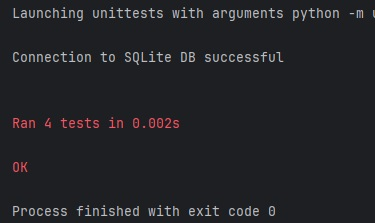
\includegraphics[width=0.6\linewidth]{images/test2}
	\caption{Результаты выполнения тестов}
	\label{fig:test2}
\end{figure}

\subsection{Интеграционное тестирование программной системы}
Каждое окно приложения представляет уникальный интерфейс, исходя из его функций.  Каждое окно, кроме главного меню, содержит виджет древа.
Древо состоит из:
\begin{itemize}
	\item столбцов с заголовками данных элементов;
	\item данных, внессённых в текущую базу;
	\item полосы прокрутки (появляется, если не все элементы древа помещаются в окно).
\end{itemize}
Главное окно включает в себя кнопки для перехода в другие окна, а также виджет переключателя режимов работы СКУД.
Основное содержимое панели управления меняется в зависимости от выбранной таблицы данных и включает в себя виджеты для изменения, удаления, добавления, поиска и просмотра данных.
Окно проверки доступа включает в себя виджеты для ввода искомых данных, кнопку проверки доступа и виджет переключения режима поиска. Пользователь может просматривать данные различных пассажиров в зависимости от выбранного режима -- <<Пассажир>> или <<Ребёнок>>.

На рисунке ~\ref{fig:example4} представлено главное меню в режиме ЧС.
Режим главного окна пользователь может изменить с помощью переключателя -- от этого будет зависеть дальнейшее поведение системы.
\begin{figure}[ht]
	\centering
	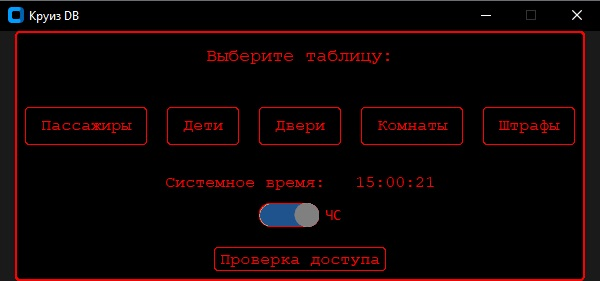
\includegraphics[width=1\linewidth]{images/Example4}
	\caption{Главное меню в режиме Чрезвычайной ситуации}
	\label{fig:example4}
\end{figure}

На рисунке ~\ref{fig:example5} представлено окно панели управления данными о штрафах и выбранным штрафом для просмотра детальной информации и последующего изменения. 
Взаимодействовать с элементом можно только тогда, когда он выбран. Его данные отображаются в соответствующих полях для этого вида данных. 
\begin{figure}[ht]
	\centering
	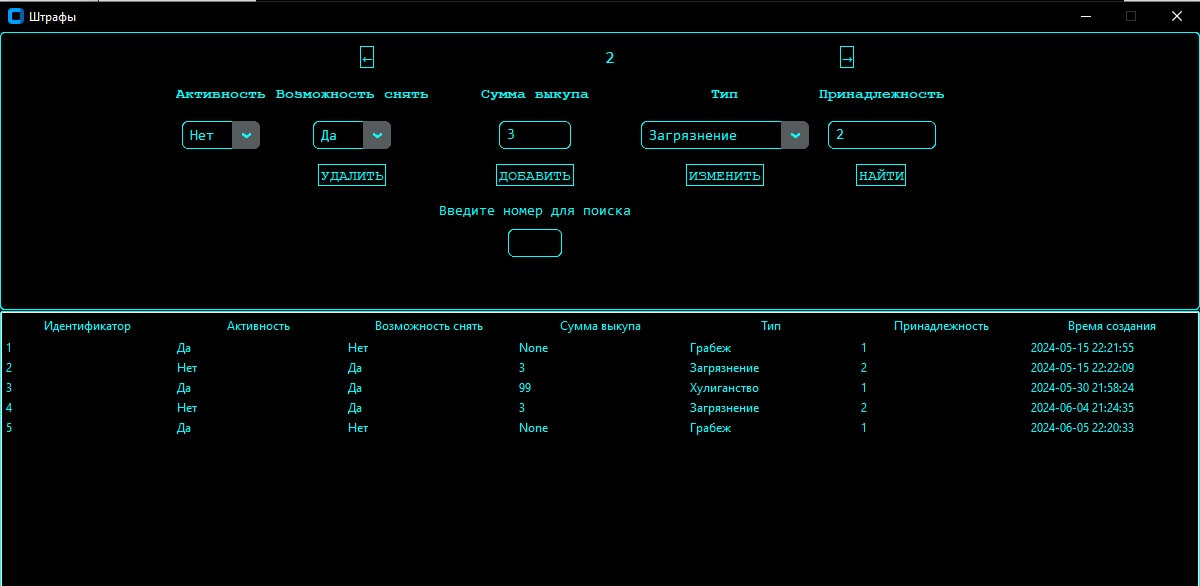
\includegraphics[width=1\linewidth]{images/Example5}
	\caption{Панель управления с выбранным элементом}
	\label{fig:example5}
\end{figure}

Менять выбранный элемент пользователь может с помощью виджета \textquotedbl стрелок \textquotedbl, расположенных в верхней части окна, или воспользовавшись опцией поиска, введя в поле \textquotedbl номер для поиска \textquotedbl идентификатор искомого элемента и нажав <<Найти>>. После чего, пользователь получит сообщение о том, был ли найден элемент.
На рисунках  ~\ref{fig:example6} и ~\ref{fig:example7} пользователь видит, что в базе есть данные о пяти штрафах и пытается найти элемент с номером идентификатором 10 и 3 соответственно.
\begin{figure}[ht]
	\centering
	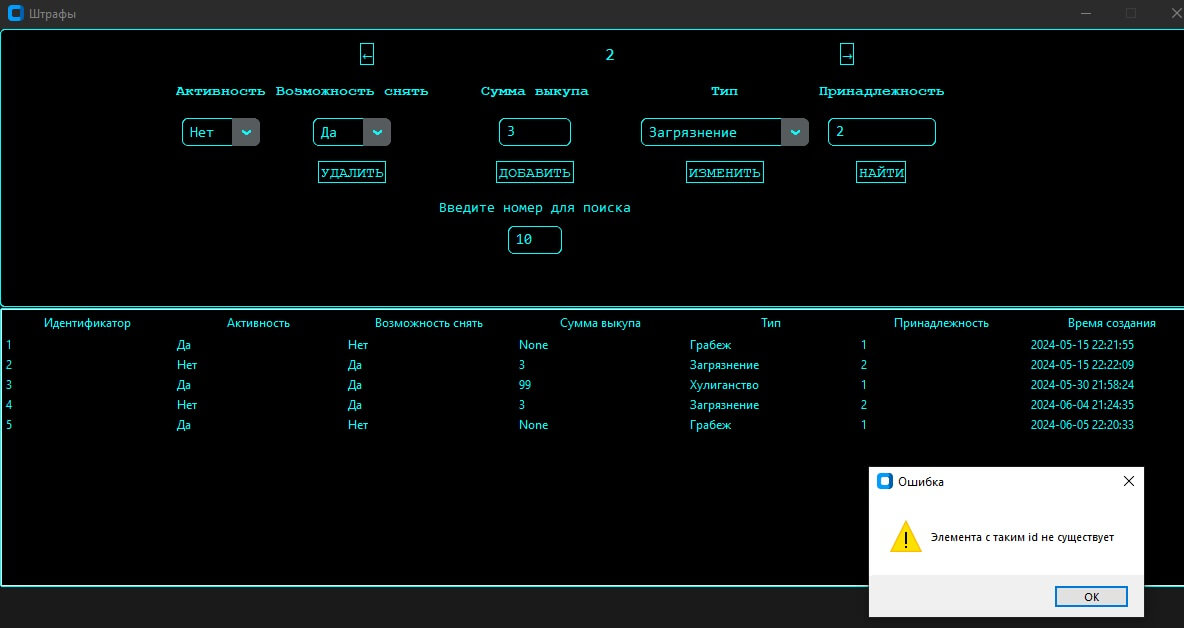
\includegraphics[width=1\linewidth]{images/Example6}
	\caption{Поиск несуществующего элемента}
	\label{fig:example6}
\end{figure}

\begin{figure}[ht]
	\centering
	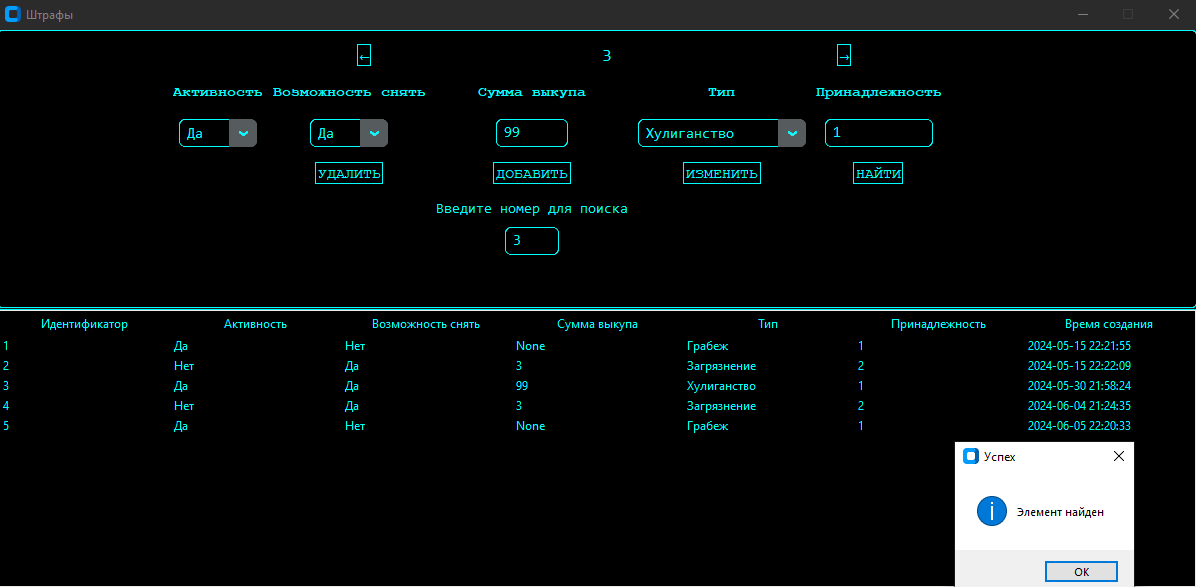
\includegraphics[width=1\linewidth]{images/Example7}
	\caption{Поиск существующего элемента}
	\label{fig:example7}
\end{figure}
В случае, когда пользователю нужно зарегистрировать новый штраф, он может добавить новый элемент, посредством заполнения всех обязательных полей и нажатием <<Добавить>>. На рисунке ~\ref{fig:example8} изображен результат добавления нового штрафа в базу.
\begin{figure}[ht]
	\centering
	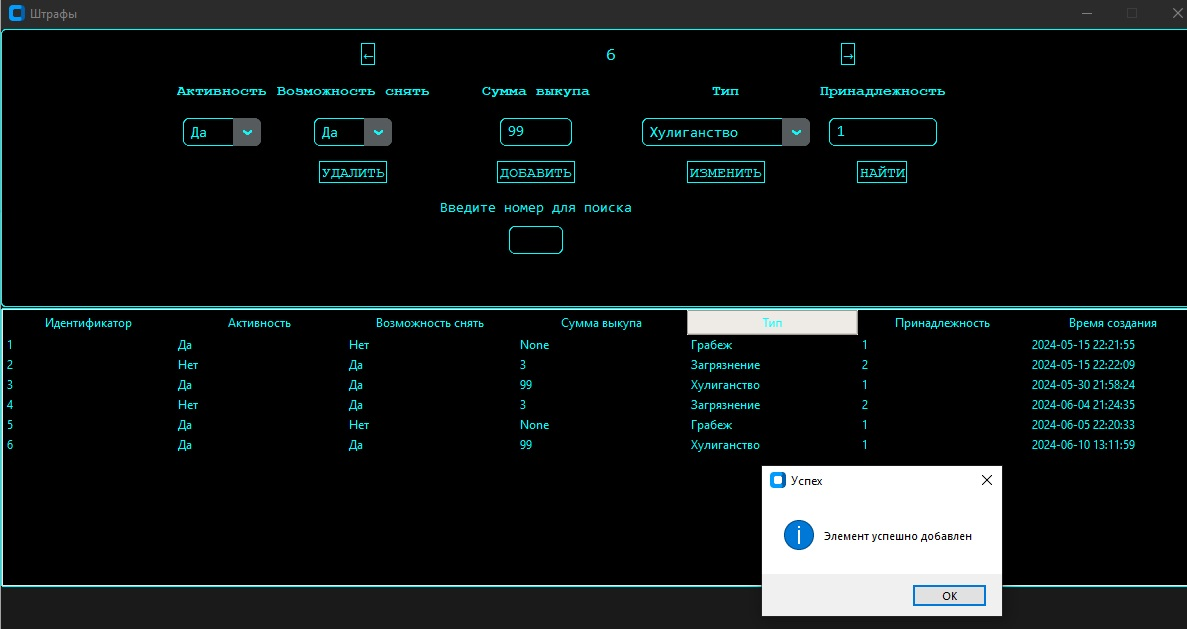
\includegraphics[width=1\linewidth]{images/Example8}
	\caption{Добавление нового элемента в панели управления}
	\label{fig:example8}
\end{figure}
Пользователь мог внести и добавить данные об элементе по ошибке. В этом случае он выбирает элемент и удаляет его, посредством клика по кнопке <<Удалить>>.
На рисунке ~\ref{fig:example9} изображён случай удаления недавно добавленного элемента.
\begin{figure}[ht]
	\centering
	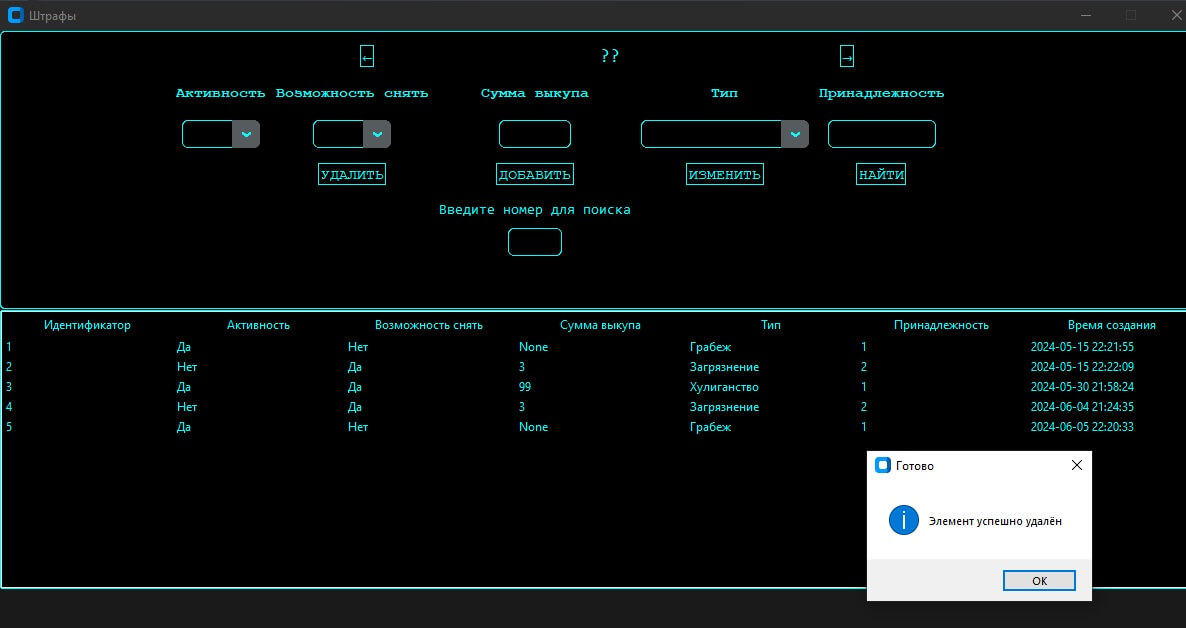
\includegraphics[width=1\linewidth]{images/Example9}
	\caption{Удаление данных о штрафе}
	\label{fig:example9}
\end{figure}

На рисунке ~\ref{fig:example10} представлена панель проверки доступа к двери, работающая в режиме <<Ребёнок>> и отражающая в виджете древа данные о доступах детей соответственно. Пользователь может переключить панель в режим <<Пассажир>> для просмотра данных о доступе пассажиров к дверям. При вводе идентификаторов пассажира и двери, и последующем нажатии на <<Проверить доступ>> пользователь получает сообщение о предоставлении доступа, принцип которого был рассмотрен в пункте 3.4 технического проекта.
\begin{figure}[ht]
	\centering
	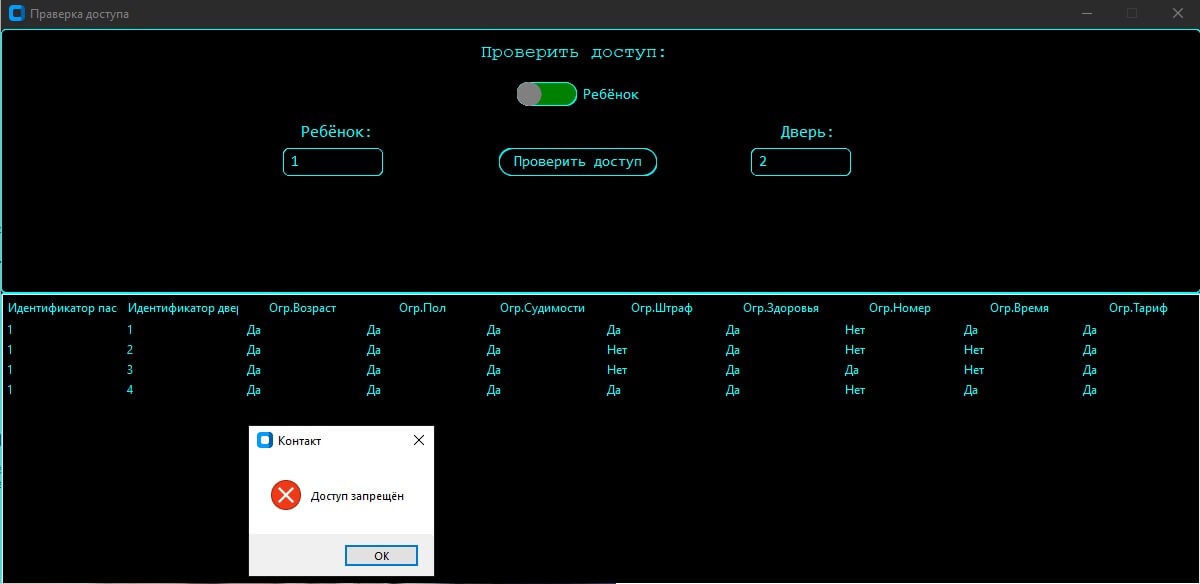
\includegraphics[width=1\linewidth]{images/Example10}
	\caption{Проверка доступа к двери}
	\label{fig:example10}
\end{figure}

\newpage
   \section*{ЗАКЛЮЧЕНИЕ}
\addcontentsline{toc}{section}{ЗАКЛЮЧЕНИЕ}

В наше время контроль доступа является сложным процессом, применяющимся для защиты мест, имущества, данных или граждан от личных до огромных корпоративных масштабов. Разработка приложения <<Программное обеспечение для системы контроля и управления доступом на круизном судне>> успешно демонстрирует применение этой технологии для контроля доступа на круизном судне.

Основные результаты работы:
\begin{enumerate}
	\item Проведен глубокий анализ предметной области, включая особенности функционирования систем СКУД на пассажирском судне.
	\item Разработана концептуальная модель и создана реляционная база данных.
	\item Разработан и реализован пользовательский интерфейс приложения, используя совместимые модули, такие как tkinter, customtkinter, sqlite3, asyncio
	\item В полной мере реализованы функции приложения, заключающиеся в контроле и управлении доступом на круизном судне.
\end{enumerate}
  
Все задачи, поставленные в начале работы, были успешно решены. Разработанное приложение соответствует всем современным требованиям и позволяет пользователю эффективно взаимодействовать в рамках контроля и управления доступом на круизном судне. 

Приложение <<Программное обеспечение для системы контроля и управления доступом на круизном судне>> может послужить основой для создания СКУД на больших объектах, где таковая требуется.

}\fi
\addcontentsline{toc}{section}{СПИСОК ИСПОЛЬЗОВАННЫХ ИСТОЧНИКОВ}

\begin{thebibliography}{9}
	
	\bibitem{dictionary}Словарь данных и система управления базами данных / Data Dictionary and Database Management System, 2019. – Текст~: электронный. URL: https://studfile.net/preview/942920/page:17/
	\bibitem{oopscdb}Бойко И. Объектно-ориентированные СУБД / И. Бойко. – Киев : Высшая школа, 2014. –- 398 с. -- Текст~: непосредственный.  
	\bibitem{security}Рыкунов В. Охранные системы и технические средства физической защиты.  /  Security Focus 2022. –- 398 с. – ISBN: 978-5-9901176-3-1. – Текст~: непосредственный.   
	\bibitem{micacc}Гринченко, Н.Н. Проектирование баз данных. СУБД Microsoft Access: Учебное пособие для вузов. / Н.Н. Гринченко и др. - М.: РиС, 2013. -- 240 c. -- ISBN: 978-5-9912-0295-4.  Текст~: непосредственный.
	\bibitem{dbrealizt}Коннолли, Т. Базы данных. Проектирование, реализация и сопровождение. Теория и практика. / Т. Коннолли. - М.: Вильямс И.Д., 2017. - 1440 c. -- ISBN:  978-5-8459-2020-1. Текст~: непосредственный.
	\bibitem{acshistory}scDataCom [Электронный ресурс] From Keys to Credentials: The History of Access Control, 2024. – Текст~: электронный. URL: https://www.scdatacom.net/blog/from-keys-to-credentials-the-history-of-access-controlnbsp
	\bibitem{dbproject}Лукин, В.Н. Введение в проектирование баз данных. / В.Н. Лукин. - М.: Вузовская книга, 2015. -- 144 c. -- ISBN: 978-5-9502-0761-7. Текст~: непосредственный.	
	\bibitem{sqlite}Medium.com. / «SQLite – Как организовывать таблицы» Автор:А.Шагин, 2020. – Текст~: электронный. URL: https://medium.com/nuances-of-programming/sqlite-как-организовывать-таблицы-81cce38af5b2
	\bibitem{umldb}Мюллер, Р.Д. Проектирование баз данных и UML. / Р.Д. Мюллер; Пер. с англ. Е.Н. Молодцова. - М.: Лори, 2013. -- 420 c. ISBN: 978-5-85-582322-6. Текст~: непосредственный.
	\bibitem{mobile}kisi [Электронный ресурс] Mobile access control guide: 2024.  – Текст~: электронный. URL: https://www.getkisi.com/guides/mobile-access-control-guide
	\bibitem{pythonprog} Васильев А.Н. Программирование на Python в примерах и задачах/ Бомбора 2023. -- 616с. --ISBN 978-5-04-103199-2 Текст~: непосредственный.    	
	\bibitem{pythonprof}Свейгард Э. Python. Чистый код для продолжающих / Питер, 2023 – 384 с. –- ISBN 978-5-4461-1852-6. -– Текст~: непосредственный.    
	\bibitem{cards}Richmond Security / Locked. Secured. Protected/ Learning About Access Control Systems: Control Cards, 2024.  – Текст~: электронный. URL: https://www.richmondsecurity.com/learning-about-access-control-systems-control-cards/
	\bibitem{OOP5}Вайсфельд М. Объектно-ориентированный подход. 5-е межд. изд. / Питер, 2024 –- 256 с. –- ISBN 978-5-4461-1431-3. – Текст~: непосредственный.    	
	\bibitem{acsspec}Британская ассоциация индустрии безопасности. Руководство по составлению спецификаций на СКУД / Второе переиздание,тираж 500 2014. -- 170 c. Текст~: непосредственный.
	\bibitem{acswork}aatel [Электронный ресурс] How do Access Control Systems work?: 2024. – Текст~: электронный. URL: https://www.aatel.com/portfolio/how-do-access-control-systems-work/	
	\bibitem{acschronicle}hidglobal [Электронный ресурс] Chronicling the Evolution of Access Control Credentials: Jim Dearing, 2021. – Текст~: электронный. URL: https://blog.hidglobal.com/2021/03/chronicling-evolution-access-control-credentials
	\bibitem{acs}Ворона В.А.,Тихонов В.А. Системы контроля и управления доступом. / Горячая Линия-Телеком 2018 г. –- 272 с. ISBN:978-5-9912-0059-2. Текст~: непосредственный.	
	\bibitem{jtkinter}python.org / Documentation: tkinter / Python interface to Tcl/Tk, 2023. – Текст~: электронный. URL: https://docs.python.org/3/library/tkinter.html
	\bibitem{async}Фаулер М. Asyncio и конкурентное программирование на Python / ДМК Пресс, 2023 –- 398 с. –- ISBN 978-5-93700-166-5. – Текст~: непосредственный.  
	
\end{thebibliography}

\ifВКР{\appendix{Представление графического материала}

Графический материал, выполненный на отдельных листах,
изображен на рисунках А.1--А.\arabic{числоПлакатов}.
\setcounter{числоПлакатов}{0}

\renewcommand{\thefigure}{А.\arabic{figure}} % шаблон номера для плакатов

\begin{landscape}

\end{landscape}
}\fi
\ifПрактика{}\else{\appendix{Фрагменты исходного кода программы}

\textbf{main.py}
\lstinputlisting[language=Python, frame=none]{code/main.py}
\newpage
\textbf{Controller.py}
\lstinputlisting[language=Python, frame=none]{code/Controller.py}
\newpage
\textbf{Tables.py}
\lstinputlisting[language=Python, frame=none]{code/Tables.py}
\newpage
\textbf{Utils.py}
\lstinputlisting[language=Python, frame=none]{code/Utils.py}
\newpage
\textbf{Validator.py}
\lstinputlisting[language=Python, frame=none]{code/Validator.py}

\ifВКР{
	\newpage
	\addcontentsline{toc}{section}{На отдельных листах (CD-RW в прикрепленном конверте)}
	\begin{center}
		\textbf{Место для диска}
	\end{center}
}\fi}\fi
\end{document}
